
\def\g4{{\sf Geant4}}

\newcommand{\codeAlgorithm}[1]{
\addcontentsline{toc}{section}{Résumé}
\begin{center}\fbox{\parbox{12cm}{\bf #1}}\end{center}}

\newcommand{\cppintro}[1]{
\lstset{language=C,
caption= #1 ,
label=listing:boundary}}

\def\cppstart{\begin{lstlisting}}
\def\cppend{\end{lstlisting}}%% Uncomment these if you write in English

\documentclass[12pt]{article}
\usepackage[english]{thesis}

\usepackage[utf8]{inputenc} % look here if scands are broken

%% Jos käytät latex-komentoa käännettäessä (oletusarvo) 
%% kuvat kannattaa tehdä eps-muotoon. Älä käytä ps-muotoisia kuvia!
%% Käytä seuraavaa latex-komennon ja eps-kuvien kanssa 
%%\usepackage[dvips]{graphicx}

%% Jos tääs käytät pdflatex-komentoa, 
%% joka kääntää tekstin suoraan pdf-tiedostoksi ja kuvasi
%% ovat esim. jpg-formaatissa tai pdf-formaatissa,   
%% käytetään seuraavaa pakettia, kommentoi siis kommenttimerkki pois
%% Huom! Tekstin marginaalit saattavat poiketa n. 2-5 mm
%% suosituksesta, jos käytät pdflatex-komentoa!
\usepackage[pdftex]{graphicx} 
\usepackage{multirow}
\usepackage{url}
\usepackage{listings}
%\usepackage{graphicx}
\usepackage[utf8]{inputenc} % look here if scands are broken
\usepackage{wrapfig}
%\usepackage{makeidx}
%\usepackage{subfig}
\usepackage{fancyhdr}
%\usepackage{asymptote}
\usepackage{amsmath}
\usepackage{verbatim} % for comment
\usepackage{eurosym} 
\usepackage{color} % for definecolor
\usepackage[colorlinks,bookmarks=true]{hyperref}

%% Saat pdf-tiedoston viittaukset ja linkit kuntoon seuraavalla paketilla.
%% Paketti toimii erityisen hyvin pdflatexin kanssa. 
%\usepackage[pdfpagemode=None,colorlinks=true,urlcolor=red,%
%linkcolor=blue,citecolor=black,pdfstartview=FitH]{hyperref}

%% Jos et jostain syystä tykkää käyttää
%% edellistä hyperref pakettia, voit käyttää myös seuraavaa pakettia
%% (tarvitaan lähinnä url-komennon määrittämiseen ja formatoimiseen)
\usepackage{url}

%% Matematiikan fontteja, symboleja ja muotoiluja lisää, näitä tarvitaan usein 
\usepackage{amsfonts,amssymb,amsbsy}  
%% paketti että saa ladottua monta kuvaa samalle sivulle.
\usepackage{subfigure}

%% Käytä seuraavaa pakettia jos haluat
%% Times-fontit LaTeX:n normaalien Computer Modern-fonttien sijaan.
%% Times-fontit ja Computer Modern-fontit ovat kummatkin roomalaisia
%% fonttityyppejä ja monet kutsuvat kaikkia roomalaisia
%% fontteja virheellisesti Times-fonteiksi,
%% vaikka tarkasti ottaen Times on vain Times-lehden fontti.
%% Computer Modern on Donald Knuthin suunnittelema fontti, joka
%% on Century Magazinen fontin variantti.
%% Huom! Kaavoihin ei tule Times-fontteja, joten lopputulos ei ole
%% välttämättä aivan tyylikäs. Pakettia ei suositella sen vuoksi. 
%\usepackage{times}  

%% Vaakasuunnan mitat, ÄLÄ KOSKE!
\setlength{\hoffset}{-1in}
\setlength{\oddsidemargin}{35mm}
\setlength{\evensidemargin}{25mm}
\setlength{\textwidth}{15cm}
%% Pystysuunnan mitat, ÄLÄ KOSKE!
\setlength{\voffset}{-1in}
\setlength{\headsep}{7mm}
\setlength{\headheight}{1em}
\setlength{\topmargin}{25mm-\headheight-\headsep}
\setlength{\textheight}{23cm}
%% Vasensuora-asettelu, joka opinnäytteessä vaaditaan. ÄLÄ KOSKE
\setlength{\parindent}{0pt}
\setlength{\parskip}{1ex}


%% Kaikki mikä paperille tulostuu, on tämän jälkeen
\begin{document}

\Language{English}{Englanti}

\university{helsinki university of technology}{teknillinen korkeakoulu}

%% Korjaa seuraavat vastaamaan omaa tiedekuntaasi
\faculty{Faculty of Information and Natural Sciences}%
{}%
%%

%% Vain kandityölle: Korjaa seuraavat vastaamaan tutkinto-ohjelmaasi
\degreeprogram{Engineering Physics and Mathematics}{}
%%

%% Vain DI- ja lisensiaatintyölle
%\professorship{Circuit theory}{Piiriteoria}
%\code{S-55}
%%

%% Valitse yksi näistä kolmesta
\degree{BSc}
%\degree{MSc}
%\degree{Lic}

%% Oma nimi
\author{Gillis Danielsen}

%% Opinnäytteen nimi tulee vain tähän
\thesistitle{Simulating carbon beam fragmentation on water phantom with Geant4}{}

%% Kandidaatintyön päivämäärä on sen esityspäivämäärä! 
%%\date{22.1.2008}

%% Kandidaattiseminaarin vastuuopettaja
\supervisor{Ph.D. Veikko Karimäki, Prof. Harri Ehtamo}{}

%% Kandidaatintyön ohjaaja
\instructor{Aatos Heikkinen}{}

%% Tehdään kansilehti
\makecoverpage

\begin{comment}
\title{Simulating carbon beam fragmentation on water phantom with the Geant4 INCL/ABLA models}

\begin{titlepage}
\pagestyle{empty}
\begin{center}
rev. 001-2009\\
\vspace{7.5 cm}
\Huge
Simulating carbon beam fragmentation on water phantom with Geant4\\

\vspace{5cm}

\Large
Gillis Danielsen, Bachelor's Thesis\\
Helsinki University of Technology\\

    \vspace{0,2cm}
  \end{center}

\end{titlepage}
\end{comment}

%% Tiivistelmän avainsanat 
\keywords{Geant4, Binary cascade, ABLA, CERN, IAEA, Hadrontherapy, Bragg peak, fragment buildup}
%% Tiivistelmän tekstiosa
\begin{abstractpage}[english]
This paper focuses on the simulation of carbon beams in a water phantom using Geant4 code as a medical application. Geant4 is a multi-purpose physics simulation package developed at CERN, Switzerland. Geant4 currently hosts multiple models suitable for the experiment, however, this paper will focus on the binary and ABLA models developed as a collaboration of scientists at CERN and many other research institutions worldwide. Results will be compared to experimental data made available by the GSI Darmstadt/E.Haettner. This work is part of the International Atomic Energy Agency(IAEA) coordinated programme to compile and evaluate charged-particle nuclear data and related Monte-Carlo codes for therapeutic applications. This work introduced extensions to the Geant4 Hadrontherapy-example, using our modelling we estimate particularly the magnitude distribution of fragment build-up at the end of the Bragg-curve.
\end{abstractpage}

%% Pakotetaan uusi sivu varmuuden vuoksi, jotta 
%% mahdollinen suomenkielinen ja englanninkielinen tiivistelmä
%% eivät tule vahingossakaan samalle sivulle
\newpage



%% Sisällysluettelo
%% addcontentsline tekee pdf-tiedostoon viitteen sisällysluetteloa varten
\addcontentsline{toc}{section}{Contents}
%% Tehdään sisällysluettelo
\tableofcontents


%% Symbolit ja lyhenteet
\mysection{Symbols and legends}

\begin{tabular}{ll}
CERN         & Organisation europeenne pour la researche nucleare \\
INCL      & intranuclear cascade, liege\\
ABLA        & Abla \\tion Abration model\\
IAEA         & International Atomic Energy Association \\
HIP        & Helsinki Institute of Physics
\end{tabular}


%% Sivulaskurin viilausta opinnäytteen vaatimusten mukaan:
%% Aloitetaan sivunumerointi arabialaisilla numeroilla (ja jätetään
%% leipätekstin ensimmäinen sivu tyhjäksi, 
%% ks. alla \thispagestyle{empty}).
%% Pakotetaan lisäksi ensimmäinen varsinainen tekstisivu alkamaan 
%% uudelta sivulta clearpage-komennolla. 
%% clearpage on melkein samanlainen kuin newpage, mutta 
%% flushaa myös LaTeX:n floatit 
\cleardoublepage
\storeinipagenumber
\pagenumbering{arabic}
\setcounter{page}{1}


%% Ensimmäinen osa, LEIPÄTEKSTI ALKAA
\section{Introduction}
\thispagestyle{empty}
%Carbon beams are a promising new alternative to traditional radiation cancer therapy. 
The history of radiation treatments dates back to 1895 when W.K.~Roentgen discovered the x-rays. It was not long before these photon rays were used to treat malign tissue. The first methods used were on today's standards very crude, and much work has gone into perfecting the treatments in order to minimize the effect of the rays on the surrounding healthy tissue and maximize the dose delivered to the malign tissue.

However, due to the statistical nature of the photon interactions, a beam of many photons is
exponentially attenuated yielding an exponential decrease of the dose with the depth. To
obtain a higher dose in the tumor than in the surrounding normal tissue, many irradiation
fields are used. The cost of this method is that a large volume of the normal tissue
will suffer from a high dose. By replacing the x-rays with high energy photons, the dose
maximum is shifted a few centimeters deeper and the exponential decrease is more shallow,
which improves the ratio between dose in the tumors and in the normal tissue. Although very sophisticated variations of the photon treatments have been perfected over time, photon therapies still produce considerable harm to the surrounding tissue. 

A much younger and less widely used technology are those of hadron- or heavy-ion based radiotherapies. Hadrons and heavyer-ions are charged particles and therefore interact with tissue in a much different way to photons. The dose-profile contains a much sharper peak due to the primary halting force being electromagnetic interaction. This peak is called the Bragg-peak, and was first discovered by William Henry Bragg in 1903.

The field of hadron treatments was pioneered at the Lawrence Berkeley Laboratory (LBL). Based on research done at the Berkeley cyclotron J.~Wilson first recomended the use of protons as a treatment method in a 1946 paper~\cite{RW46}. Furthermore, the first de facto treatment was administered at Berkeley in 1953. Today there are a number of proton-based therapies in clinical use all around the world, for example in Harvard General Hospital (see fig). %fixme
\begin{figure}[h]
\begin{center}
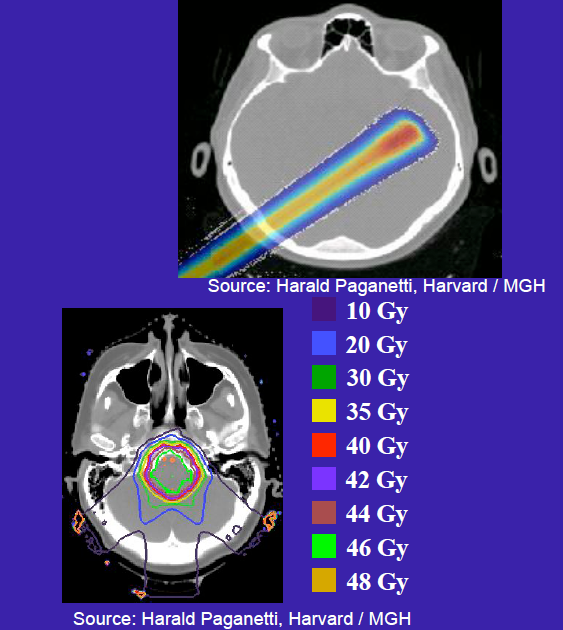
\includegraphics[height=9cm]{images/HarvardHadronTreatment.png}  
\caption{\label{fig:HarvardHadron} Example of Geant4 proton treatment simulation visualized.} 
\end{center}
\end{figure} 
Heavy-ion therapies have remained considerably less common and have remained on a more experimental level. Clinical trials were conducted at LBL inbetween 1977 and 1993 with $^{20}$Ne. At the end of 2008 the Particle Therapy Co-Operative  Group (PTCOG) estimated that more than 7000 heavy-ion treatments had been conducted at treatment facilities it monitors worldwide. Treatments based on $^{12}$C beams have been offered at NISR in Japan and in Germany at GSI~\cite{PTCOGstat}. Carbon beams is currently the most active and promising area of heavy-ion therapy research. 

The motivations for heavy-ion treatments as an alternative or complement to hadron treatments are considerable. Firstly carbon ions have the added advantage of higher ionisation-density at the end of their range, causing greater correlated damage to the DNA-structure of a single cancerous cell and therefore induces damage in a way that makes it less likely the cell is able to repair. In a 2008 article O.~Jäkel~\cite{ojakel} approximates the beam's increase in biological efficiency by a factor between 1.5 and 3 in comparison to proton treatment depending on the application. Secondly, Heavy-ions ions are less scattered in lateral directions which yields better dosage control in many applications. However, the tradeoff is that carbon-ions will fragment into smaller particles, yielding an unwanted ``tail`` to the energy-loss profile. One of the main motivations of the work is to study this ''tail'' for the ``worst case scenario'' of 400 MeV - an upper limit in medical applications.

A number of data-sets are available for carbon beams. This paper will be compare data to beam-measurments by E.~Haettner as a part of her master's thesis~\cite{ehaettner}  at the GSI facility in Darmstadt, Germany. This paper reproduces the experimental setup used by E.Haettner as a computer simulation model. The aim of this paper is to provide good reference data for the standardization work involved in hadron treatment. Furthermore, this paper evaluates the feasibility of the Geant4 models for such simulations by comparison to experimental data. This benchmarking is part of IAEA's INDC International Nuclear Data Committee and Heavy Charged-Particle Interaction Data For Radiotherapy project which compares different Monte-Carlo codes~\cite{SummaryReport}.\footnote{Bachelor's thesis produced in the framework of the Finnish CERN Summer Training 2009. Supervisors A.~Heikkinen and V.~Karimäki from Helsinki Institute of Physics and H.~Ehtamo of Helsinki University of Technology} %fixme footnote

%% Opinnäytteessä jokainen osa alkaa uudelta sivulta, joten clearpage
\clearpage
\section{Theory}

\subsection{Electromagnetic physics of Bragg-curve}
As charged particles penetrate tissue they interact with the tissue through elastic and inellastic collisions with the electrons and nuclei, eventually loosing all of their energy. The most typical interaction is that of inelastic collisions with electrons, contributing as much as 99\% of the total energy loss.

The beam's energy loss $dE/dx$ as a function of depth results is described by the Bragg curve (see fig). %fixme
 Theoretical estimates for this relation have existed since the first classical treatment by Bohr in 1913~\cite{bohr13}. The currently used quantum model was derived by Bethe and Bloch in 1953~\cite{bethebloch53}  and is commonly known as "Bethe's stopping power formula". The Bethe stopping power formula is considered a good model for most fast (E>...) %fixme larger than something
charged particles, with the exception of electrons.

\begin{equation}
 \frac{dE}{dx} = \frac{4 \pi}{m_e c^2} \cdot \frac{nZ^2}{\beta^2} \cdot \left(\frac{e^2}{4\pi\varepsilon_0}\right)^2 \cdot \left[\ln \left(\frac{2m_e c^2 \beta^2}{I \cdot (1-\beta^2)}\right) - \beta^2\right],
\label{bethebloch}
\end{equation}
where $\beta = v/c $, 
$v$ is the velocity of the particle,
$E$ is the 
energy of the particle,
$x$ is the 
distance travelled by the particle,
$c$ is the 
speed of light,
$Z$ is the 
particle charge,
$e$ is the 
charge of the electron,
$m_e$ is the 
rest mass of the electron,
$n$ is the 
electron density of the target and 
$I$  is the 
mean excitation potential of the target.


However, as the speed of the particle has decresed to the order of magnitude of the Bohr velocity the nuclear charge $Z$ will no longer remain constant and has to be aproximated by the effective charge, given by the Barkas formula. $$Z_{eff} = Z(1-e^{-125\beta_{P}Z})$$

In this theoretical model the form of the Bragg-peak can be visualized as the $1/v_{p}^2$ relation increases the energy-loss as speed decreases. However, the effective charge will decrease at an exponential rate, thus, converging the Bragg-curve.

Particles penetrating matter do not only deposit energy through inelastic electron collisions, they might as well be involved in nuclear reactions and fragmented. A common simple model for explaining this is called the abrasion-ablation model. In this model high energy projectiles can be described as particles that move on straight lines through the
target. From time to time a target nuclea lie on this line, thus causing a collision. Bullet
and target nucleons which overlap eachother in this model (see fig~\ref{fig:ablationabration}) are called participants. The remaining parts of the projectile and target nucleus are called spectators. The momentum of the spectators in the projectile and target are only slightly affected by the collision. The participant nucleons form an excited entity, ``a fireball'', which fragments into separate light ions or single nucleons.
The Wilson-model %fixme physics reference manual reference here
that also provided in Geant4 features a physics model more reminiscient to this approach. This kind of a model is however not directly comparable to the model used in this paper through INCL and ABLA.
\begin{figure}[h]
\begin{center}
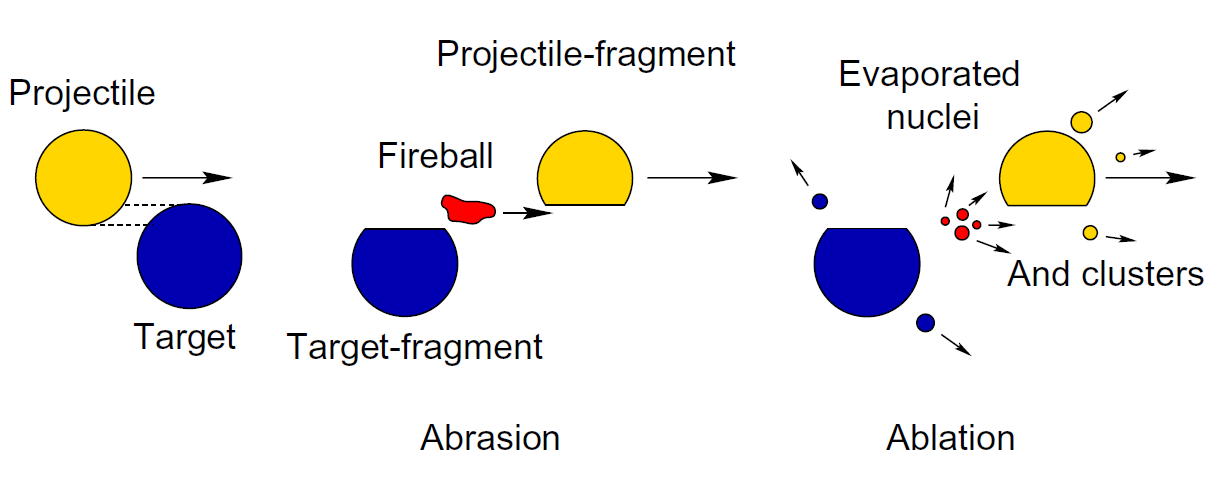
\includegraphics[width=0.8\textwidth]{images/ablationabration.png}  
\caption{Schematic description of the Wilson abration-ablation model in Geant4.}
 \label{fig:ablationabration}
 \end{center}
 \end{figure}



\subsection{Intranuclear cascade and fission/evaporation} %theory, no practical aspects

INCL4 is a Monte-Carlo type Intranuclear Cascade Model, whereas ABLA is the the complementing Monte-Carlo evaporation/fission model. In practice this means INCL is used to determine what happends just after the the projectile particle hits the target nucleus, while ABLA is used to determine what nuclear process is caused through the following excitation of the target due to the collision event. It is notable that the time-frame for evaporation and fission events are orders of magnitude greater compared to the events modelled by INCL.

\begin{figure} 
\begin{center}
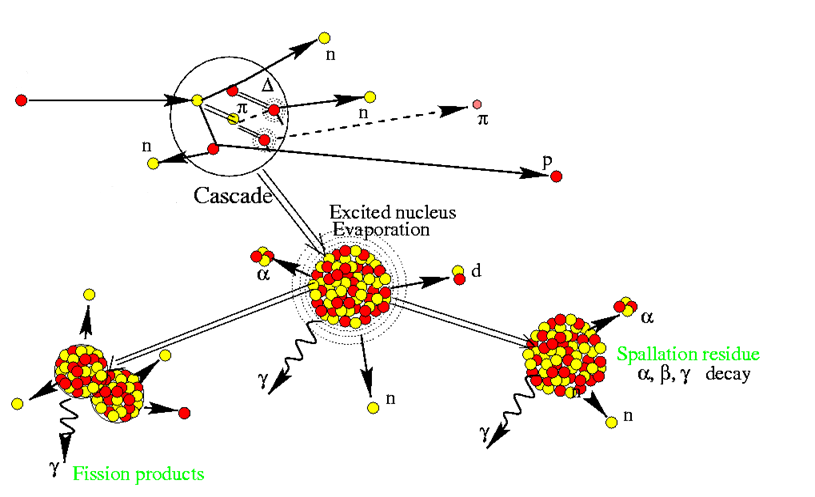
\includegraphics[width=0.8\textwidth]{images/inclScematic.png}  
\caption{\label{fig:inclschematic} Schematic diagram of INCL and ABLA models.}
 
 \end{center}
 \end{figure}

\subsubsection{Binary cascade}
The binary cascade is a hybride cascade model with certain aspects of a quantum mechanical dynamics model. The model is characterized by being based on binary scatterings between reaction participants and nucleons within the nucleus.

In this model the nucleons are described as gaussian wave packages, a nucleus is then built up by combinations of these wave-packages. However, the Slater determinant is ignored.


\begin{equation}
\Phi(x,q_i,p_i,t) = \frac{2}{(L\pi)^{\frac{3}{4}}}exp((-2/L(x -q(t)))^2+ip_i(t)x)
\label{wavePackage}
\end{equation}


The 3-dimensional nucleus model in the binary cascade assumes a isotropic spherical nucleus. The nucleus density is then describedby a Woods-Saxon potential for heavy Ions. Lighter ions are described through a harmonic oscillator nuclear shell model. Almost all ions involved in the simulation in this paper are considered light by this definition. These distributions are 

\begin{equation}
\rho(r) = 
\begin{cases}
\begin{cases}
(\pi R^2)^{\frac{3}{2}}exp(-r^2/R^2) & \text{A}<16 \text{ (Harmonic oscillator)}\\
\frac{\rho_{0}}{1+\exp({\frac{r-R_{0}}{a}})} & \text{A}>16 \text{ (Woods-saxon)}
\end{cases} & r < R_{max} \\
0 & r > R_{max} \\
\end{cases}
\label{binaryCascadePotential}
\end{equation}

The nucleons are then randomly distributed from these probability densitydistributions. The Fermi-momentum for a nucleon is then decided according to the Thomas-Fermi approximation $p^{max}_F(r) = \hbar c (3 \pi^2 \rho(r))^\frac{1}{3}$. $A-1$ nucleons are then given a momentum between zero and the Fermi momentum. The last momentum is choosen so that all momentums even out by picking the negative sum of all other momentums. If this momentumn happends to be above the Fermi momentum other momentums are repicked randomly until a satisfactory configuration is available.

The binary cascade transportation algorithm starts by picking randomly the impact parameter from a disc which is perpendicular to the distance vector inbetween the center of the disc and the middle of the nucleus. The closest distance $d^{min}_{i}$ by straight-line trajectories are calculated for each nucleon in the stochastically generated nucleus. The binary cascade then proceeds to calculate the interaction cross-sections $\sigma_i$ with all target based on the momenta of the nucleon in the nucleus, and the projectile momentum. Nucleons that have a smaller interaction radius than their distance $d^{min}_{i}$ are considered as plausible interaction targets. The plausible interaction targets are listed accoring to their individual time-of-flight by straight-line trajectory $t^{tof}_i$. The primary particle is then transported in the nuclear field with steplengths in the magnitude of the difference between the different times of flight $t_{step} = t^{tof}_i - t^{tof}_i+1$. The equations of motion are solved in the nuclear field by integration with Runge-Kutta approximation. If no collision between the primary and any nucleon is found a new nucleus and impact parameter is picked.
%fixme, below could be better formulated
Nucleon-nucleon interactions are then based on experimental data and phenomenology. After collisions secondaries of the collision that are Pauli allowed and above the Fermi momentum $p_F$ are traversed as new primaries. The Binary cascade does however not consider collisions inbetween participants.
%humm, why do we care about this if they are below fermi mometum anyway? or do we mean the different primaries?

The Binary cascade model proceeds as long as there are still particles above the kinetic energy threshold  of 75 MeV. The cscade model is also stopped if the mean kinetic energy of the participants has dropped below a second threshold (15 MeV). Once this phase is reached the nucleus is handed to the evaporation model.

\subsubsection{Geant4 evaporation model}

Once the cascade model has reached one of its cut-off criteria the remaining excited nucleus is passed on to the evaporation model which is a more statistical model based originally on the work of Weisskopf \ref{Weisskopf}. In this model the nucleus is assumed to be in an equilibrium state.

For light-nucleons a Fermi-break-up is possible if the nucleus type satisfies $A < 12$ and $3(A - Z) < Z < 6$ and furthermore has an excitation energy three times as large as its binding energy.

The evaporation model takes the nucleuses parameters as input. On the basis of this data statistical distribution is served and monte-carlo picked events are decided.


\subsubsection{Fermi break-up}

For light nuclei the excitation energy is often of the magnitude of the nucleon binding energy. Therefore it is possible to construct rather simple predictive statistical models for break-up. This approach was first introduced by Enrico Fermi and is thus called the Fermi break-up model. It is applied to all nucleuses with $A < 17$ that have suitable excitation. %fixme: phase space should be mentioned

\subsubsection{Fission model}

The Geant4 fission model utilizes the empirically found relation that the distribution of fragments from a fission process has both a syummetric and an antisymmetric component, defining the total fission output as.
\begin{equation}
 F(A_f) = F_{sym}(A_f) + \omega(U,A,Z) F_{asymm}(A_f) 
\label{fissionSymmetricAsymmetric}
\end{equation}
Where $\omega$ defines the relative contribution of each component and is a function of the excitation energy U, and the atomic numbers of the fissioning nucleus.

From experimental data it has been found that good approximations for the functions $F_{sym}$ and $F_{asym}$ can be acquired with exponential fits on $A$ and $A_f$ as variables.

At given mass of fragment $A_f$ the experimental data on the charge $Z_f$ was found to be well described by a Gaussian fit. The average kinetic energy is described through the empirical relation $<T_{kin}>=0.1178Z^2/A^\frac{1}{3} + 5.8$. However, it is also known and accoutned for that the kinetic energy distribution of the asymmetrically scattered fission products are larger than that of the symmetrically distributed ones. 

For further discussion of the Geant4 fission model the reader can consult the Geant4 physics reference manual~\cite[Chap 31.]{physicsManual}.

\section{Simulation setup} %practical aspects of simulation
The simulation is performed with the latest versions of the Geant4 suite version 4.9.3b with the newest simulation models available in the distribution.

The simulation code was based around the hadrontherapy simulation produced by G.A.P. Cirrone, F. Di Rosa, S. Guatelli and  G. Russo of INFN Genova and Catania. The aim was that that this IAEA benchmark simulation could be distributed alongside the hadrontherapy example. This however required rewriting the code at various places. Major changes in the code included.

Analysis was to be done in ROOT bypassing AIDA that is used by the hadrontherapy example.

The geometry had to be rewritten, but in such a way that it may be interchangeable through macro commands. Reqriting the geometry also meant having to rewrite some of the detection code.

Multiple runs needed to be able to be run.


\begin{figure}[ht] 
\begin{center}
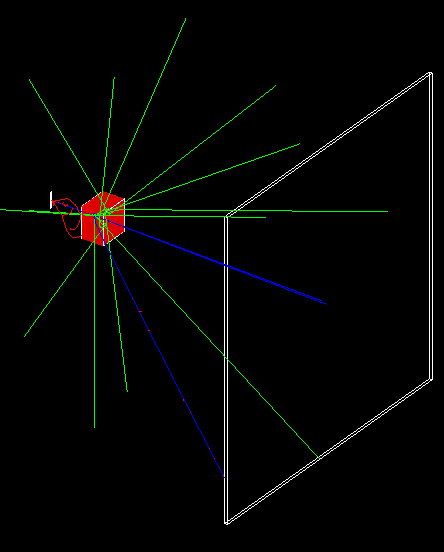
\includegraphics[width=0.5\textwidth]{images/oneEvent.png}  
\caption{\label{fig:oneEvent} OpenGL visualization of one event with 27.9cm thick water-phantom.}
\end{center}
\end{figure}

\begin{figure}[ht] 
\begin{center}
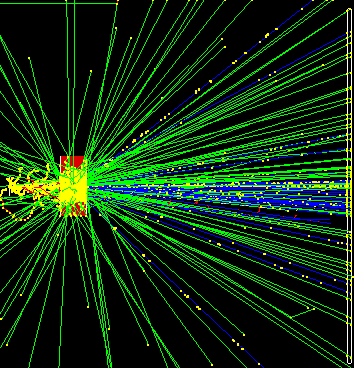
\includegraphics[width=0.5\textwidth]{images/twentyEvents.png}  
\caption{\label{fig:twentyEvents} OpenGL visualized profile view of the simulation with the tracks recorded from 23 incident events. This clearly visualizes the yield of fragments has a clear forward directed distribution.}
\end{center}
\end{figure}


\subsection{Characterization of the primary beam and experimental setup for the
IAEA benchmark}

Reference data for the measurements involved in this paper have been acquired from E. Haettner ~\cite{ehaettner}  Haettner performed these measurements at the GSI facility in Darmstadt, Germany. Haettner's experimental setup is presented below. Haettner used two different setups for the measurements made with the H1 detector and the MWPC detector used for calculating the Bragg-curve.

\subsubsection{H1 measurements}

The figure ~\cite{fig:haettnersetup3} shows the geometry Haettner used in angular and energy distribution measurements. This setup was recreated as well as possible  in the simulation environment. The major differences being:
\begin{itemize}
\item the pipe in the water-phantom was by inspection of photograph \cite{fig:haettnersetup2} deemed impossible to recreate in such a way that it could be assumed to recreate any backscattering effects or similar induced by the pipe.
\item The water phantom had the cross-section of 50x60cm. However, the beam exit-window had only an area of 32x8 cm. It was assumed that the detector was during angular experiments moved in the horizontal plane (the broader side of the window) and thus it was deemed a fair assumption to use a water-phantom with a cross-section of 32x32cm in the y-z plane. 
\item the detector itself was changed into a large scoring plane registering all incoming particles. The measurements themselves were then analysed through this data in ROOT. This allowed to minimize the amount of time-consuming simulation-runs by assuming symmetric fragmentation.
\end{itemize}

\subsubsection{Bragg-Curve measurements}
In this paper the bragg-curve is counted by imaginary voxel-layers in the phantom, and therefore is only for interest in compensating the water equivalents added by Haettner into the results for the different parts of the experiment.

This means that data acquired through the simulation technique used should be augmented by a water-equivalents for the non-water elements approximated by haettner in~\cite[table 4.1]{ehaettner}. The sum of which is an water-equivalent of 0.578 cm.



\subsection{Geometry}

\begin{figure}[!h] 
\begin{center}
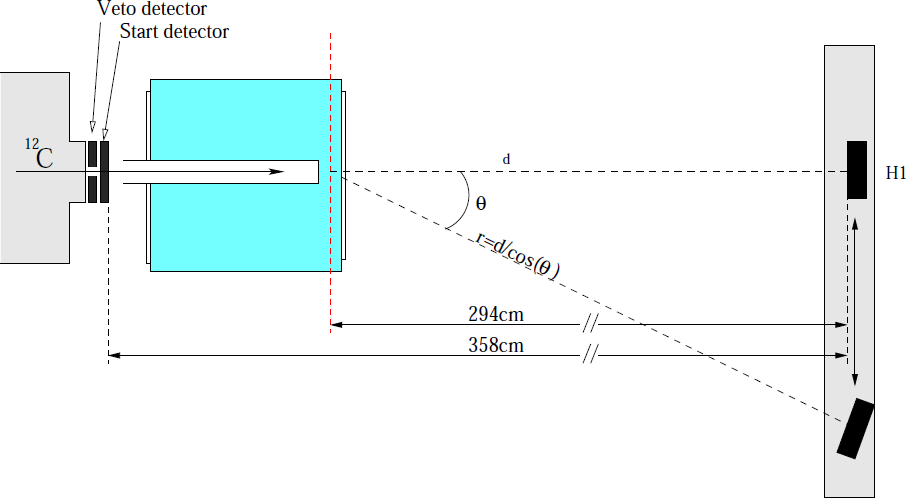
\includegraphics[width=0.9\textwidth]{images/haettnersetup3.png}[h]  
\caption{\label{fig:haettnersetup3} E.Haettner's experimental setup for measurements made with the H1 detector. In this paper and the simulation-code the angle denoted by Haettner with $\theta$ is denoted $\phi$.}
 \end{center}
 \end{figure}


\begin{figure}[!h] 
\begin{center}
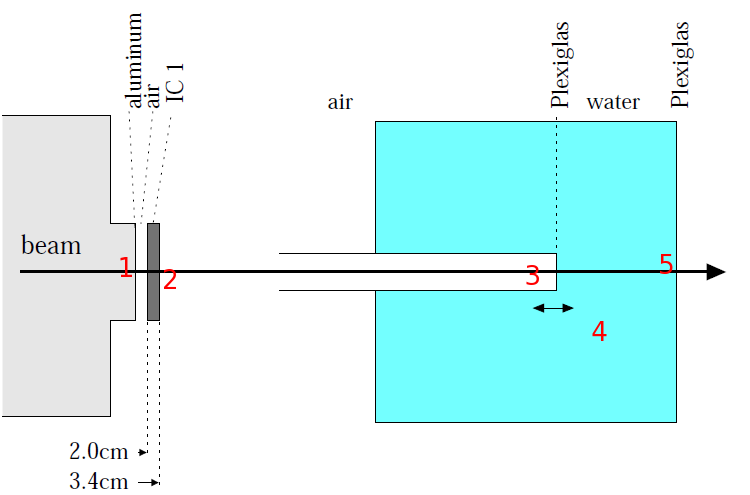
\includegraphics[width=0.9\textwidth]{images/haetnnersetup2.png}[h]  
\caption{\label{fig:haettnersetup} E.Haettner's experimental setup for calculation of Bragg peak.}
 \end{center}
 \end{figure}
\begin{figure}[ht] 
\begin{center}
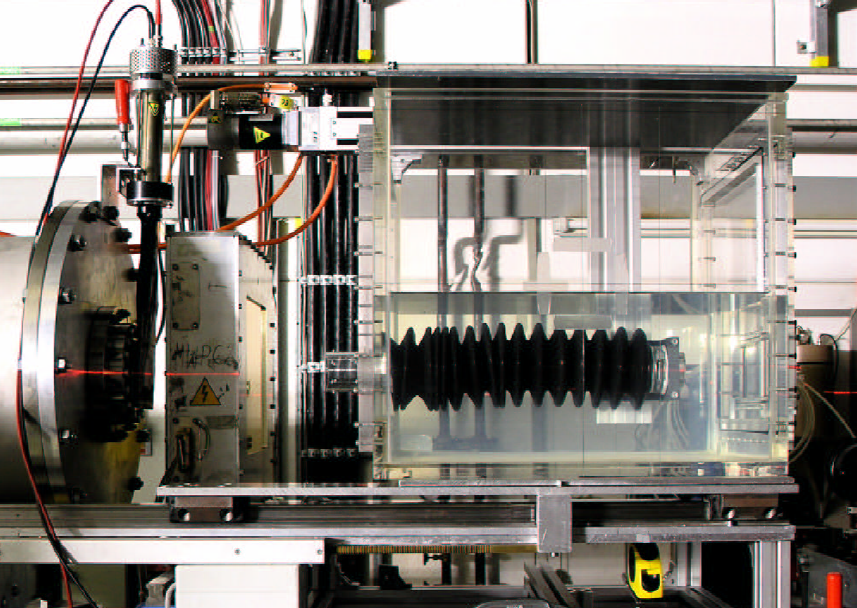
\includegraphics[width=0.9\textwidth]{images/haettnersetup.png}[h]  
\caption{\label{fig:haettnersetup2} E.Haettner's experimental setup photographed.}
 \end{center}
 \end{figure}

 \begin{table}[h]
\begin{tabular}{lllll} %fixme:
 & & & \textbf{200MeV} & \textbf{400 MeV} \\
1&Beam source window &\textbf{Aluminium}&0.1mm& 0.1mm\\
2&Ionization Chamber 1 &\textbf{Air-equivalent}&1.4cm& 1.4cm\\
3&Adjustable tube window &\textbf{Plexiglas}&2mm&2mm\\
4&Phantom &\textbf{Water}&0-40cm& 0-40cm\\
5&Container back-window &\textbf{Plexiglas}&2mm&2mm\\
6&Ionization chamber 2&\textbf{Air-equivalent}&3.7cm& 3.7cm\\
\end{tabular} 
\caption{\label{fig:SimSetup} The 1-d thicknesses of materials in the beam'a path. The experimental setup was deemed impossible to recreate as to account for the effects of the true 3-d structures in the experiment.}
\end{table}


%\begin{figure}[ht] 
%\begin{center}
%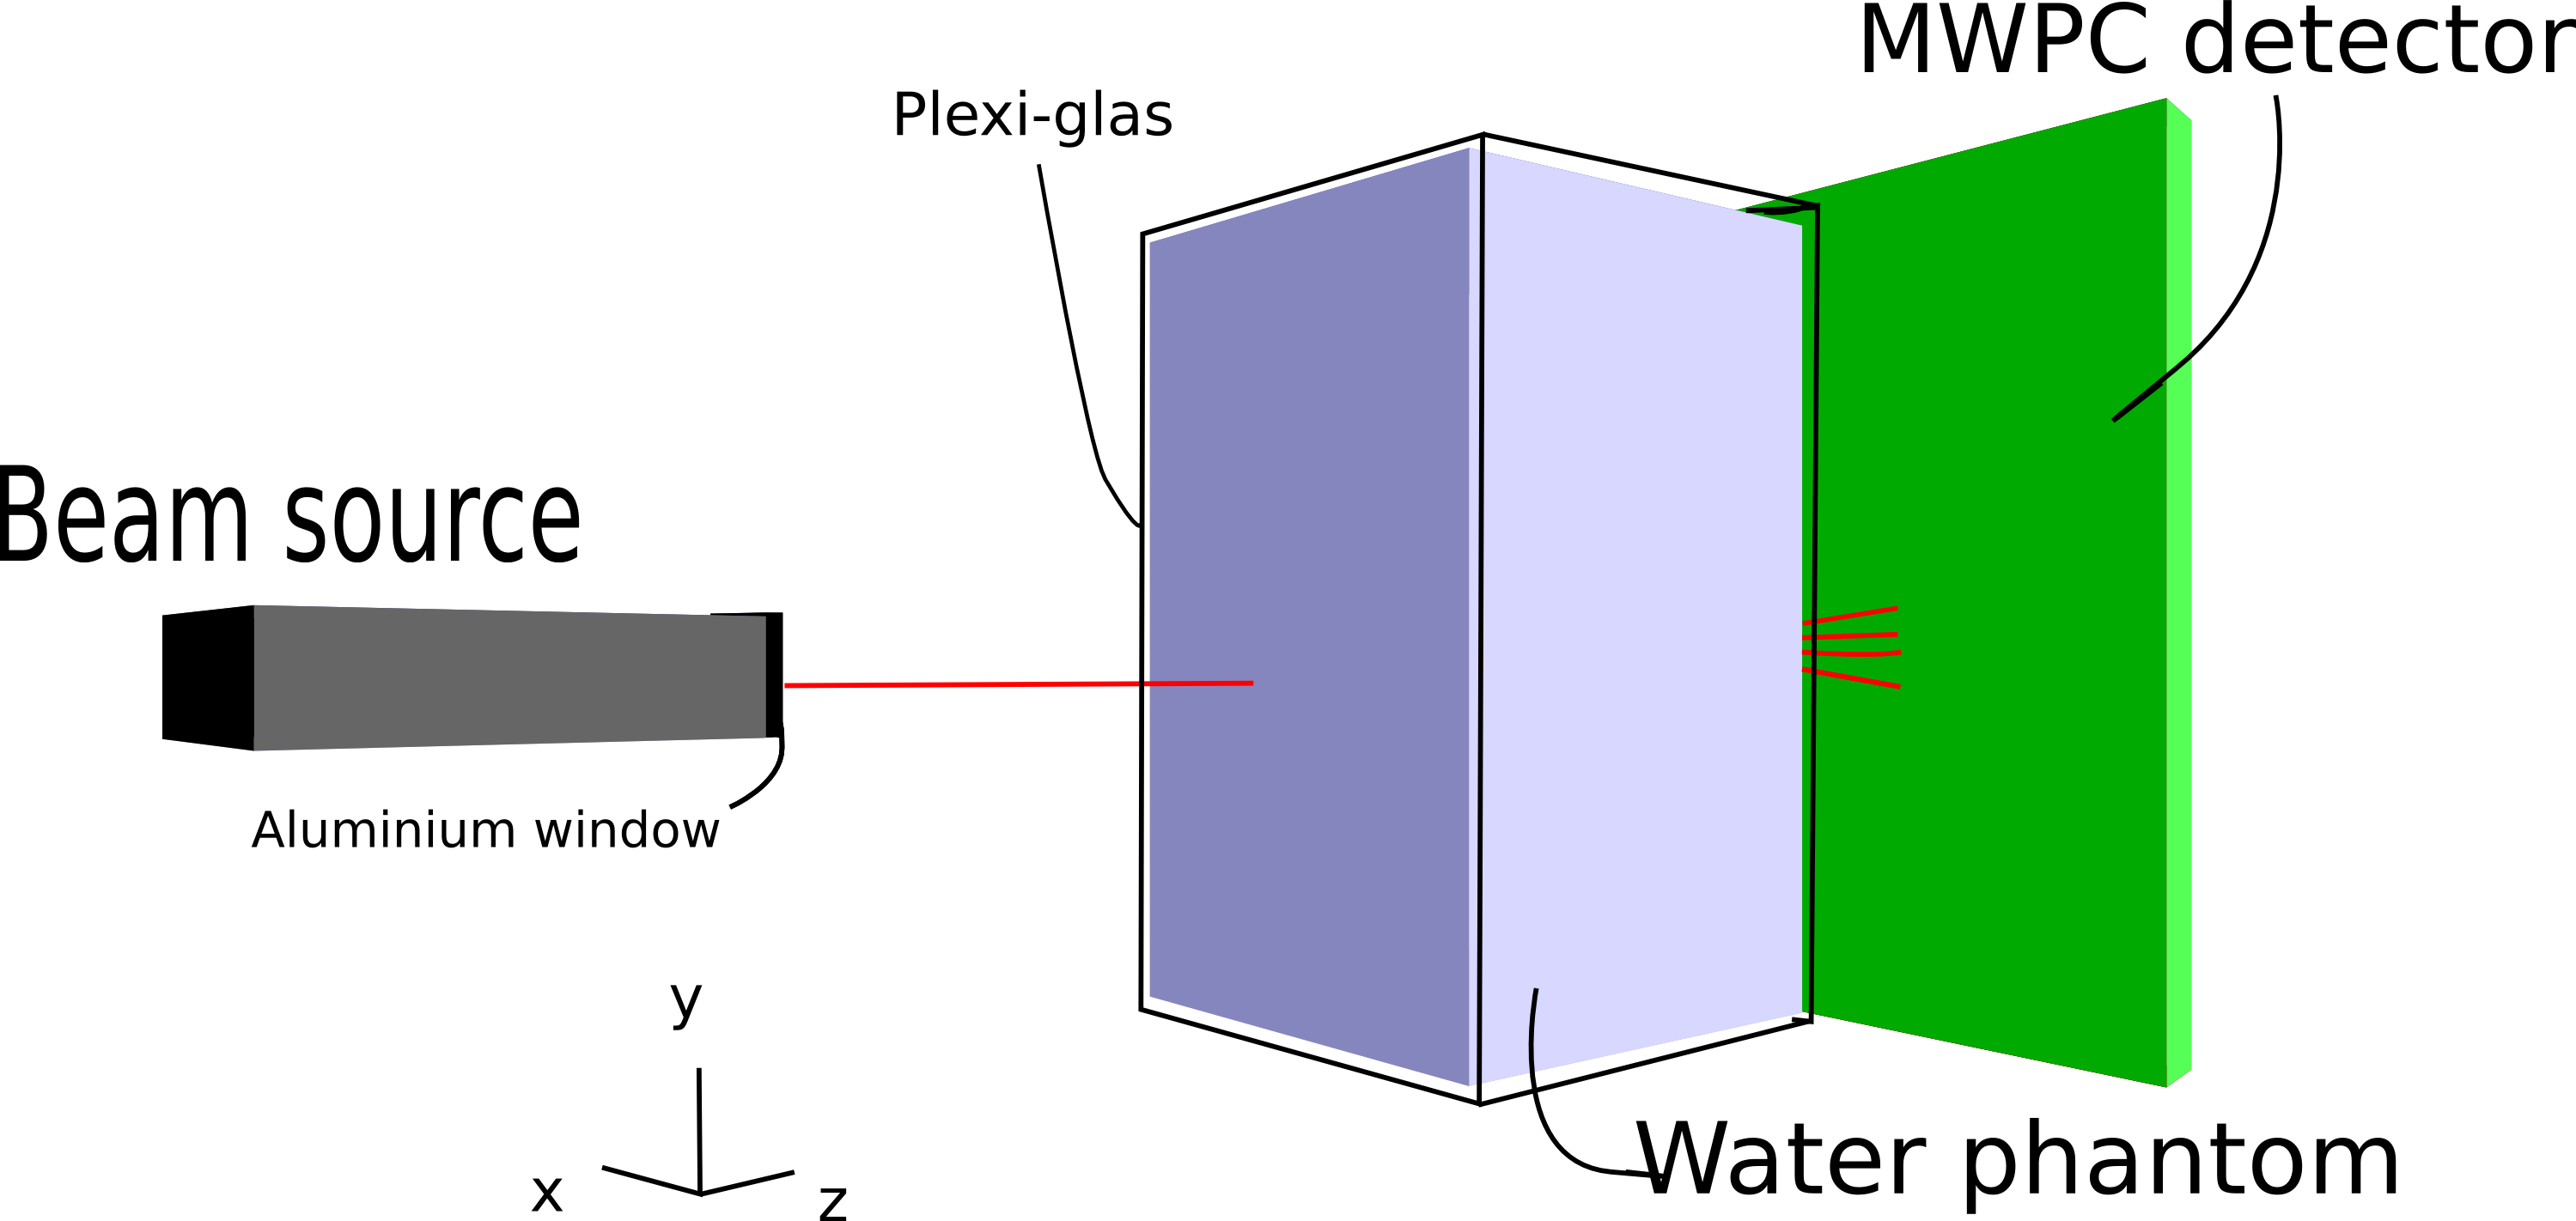
\includegraphics[width=0.9\textwidth]{images/SimSetup.png}[h]  
%\caption{\label{fig:SimSetupIncscape} A simplified illustration of the simulation-setup. A beam passes an %adjustable water-target and scatters. The scattering is measured by a simulated MWPC-detector.}
 %\end{center}
 %\end{figure}

%\begin{table}[h]
%\begin{tabular}{lllllll}
% & \textbf{200MeV} & & \textbf{400 MeV} & & \\
% &\textbf{thickness}&\textbf{mass / a.u.}&\textbf{WE}&\textbf{thickness}&\textbf{mass / a.u.}&\textbf{WE} \\
%\textbf{Aluminium}&0.1mm&0.027 $g/cm^2$& 0.027cm& 0.1mm&0.027 $g/cm^2$&0.027cm\\
%\textbf{Air and IC}&72cm &0.073 $g/cm^2$& 0.073cm& 91cm&0.109 $g/cm^2$&0.092cm\\
%\textbf{Plexiglas}&4mm&0.478 $g/cm^2$& 0.478cm& 4mm&0.476 $g/cm^2$&0.478cm\\
%\textbf{Water}&26.89cm&26.89 $g/cm^2$& 26.89cm& 8.04cm&8.04 $g/cm^2$&8.04cm\\
%\textbf{TOTAL}& &27.47 $g/cm^2$& 27.46 cm& &8.65 $g/cm^2$&8.64cm\\
%\end{tabular} 
%\caption{\label{fig:SimSetup} The 1-d thicknesses of materials in the beams path, ignoring effects induced by the true 3d-structure.}
%\end{table}


%\begin{center}
% \begin{table}[h]
%\begin{tabular}{llll} %fixme:
%& & \textbf{200MeV} & \textbf{400 MeV} \\
%Beam source window &\textbf{Aluminium}&0.1mm& 0.1mm\\
%Lab and IC's &\textbf{Air}&72cm& 91cm\\
%Water-container &\textbf{Plexiglas}&4mm& 4mm\\
%Phantom &\textbf{Water}&26.89cm& 8.04cm\\
%Beam source window &\textbf{Aluminium}&0.1mm& 0.1mm\\
%Lab and IC's &\textbf{Air}&72cm& 91cm\\
%Water-container &\textbf{Plexiglas}&4mm& 4mm\\
%Phantom &\textbf{Water}&26.89cm& 8.04cm\\
%\end{tabular} 
%\caption{\label{fig:SimSetup} The 1-d thicknesses of materials in the two beams' paths at the Bragg-peak. This presentation ignores %effects induced by the true 3d-structure.}
%\end{table}
%\end{center}



\begin{figure}[h] 
\begin{center}
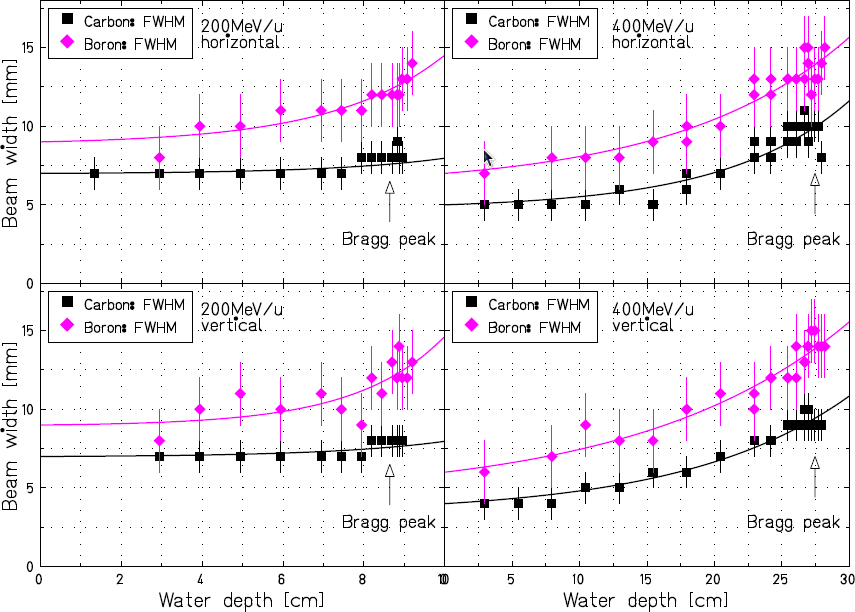
\includegraphics[width=0.9\textwidth]{images/haettner48.png}  
\caption{\label{fig:haettner48} Haettner's experimental measurements of the relation between the depth in water and FWHM of different nucleons.}
 \end{center}
 \end{figure}

\subsubsection{Beam shape}

%0.2^2/(3+0.279/2)^2

The beam is considered a pen-shaped beam. Haettner has performed several measurments to characterize the beam's accuracy. These results have to be reproduced in the simulated beamline correctly, and are thus evaluated in the thin-target experiment. Haettner produced the relation ~\ref{fig:haettner48} for the depth in water and the FWHM of the beam.

Haettner evaluates the accuracy of the beam's energy to be $\frac{\Delta E}{E}\approx5*10^{-3}$, meaning that the energy distribution of the beam is very narrow. This error was simulated with a gaussian distribution with the standard deviation 1 meV/u and 2MeV/u for the 200 respectively 400 MeV Beams.

In this simulation the beam is reproduced at the beam source (see ~\cite[1]{fig:SimSetup}) as measured by Haettner with no phantom and zero distance from start detector to the last detector. The beam is measured right after the beam-source window. The beam-source itself is assumed to produce a paralell beam. The first source of scattering the beam is the aluminium window of the beam-source, but as this measurement is made right after the window it can be used to characterize the paralell beams width. However inspecting further measurements at 1 and 3 meters show the effects of scattering in the aluminium, detectors and air as a broadening beam. The scattering of the beam is considerably different depending on the energy of the beam.

The beam width however has a distribution with an FWHM of 4mm which needs to be accounted for. Assuimng a normal distribution this meant adding a standard deviation of 1.7mm according to the relation $\mathrm{FWHM} =   2 \sqrt{2 \ln 2 } \; \sigma \approx 2.35482 \; \sigma$.

Furthermore, in this paper the scattering in air by a paralell beam could not be fullfillingly reproduced with the models used. Thus, a small gaussian deviation in the beams direction vectors z and y components were introduced (see \cite{beamShapeAnalysis}).

E.Haettner proceeds to analyze the scattering of the beam with variable water thicknesses, shown in figure ~\ref{fig:haettner48}.

\subsubsection{Water tank}
The water phantom had in the experiment the cross-section of 50x60cm. However, the beam exit-window had only an area of 32x8 cm, and the physical parameters of what covered other parts was unknown. Therefore it was assumed that the detector was during angular experiments moved in the horizontal plane (the broader side of the window) and thus it was deemed a fair assumption to use a water-phantom with a cross-section of 32x32cm in the y-z plane. This regrettably makes it impossible to study backscattering and similar effects with high precision.

\subsubsection{Beam attenuation}

In order to calculate the Bragg Curve of the beam the previous experiment a set-length water-phantom of 40 cm was placed in the path of the beam as illustrated. The amount of water was approximated on the basis of E.Haettner's work so that the entire bragg-curve and a considerable part of the fragment-tail would be visible. This water-phantom was divided into 1x1x400 primitive scoring voxels. This in effect means the water-phantom was presented as 400 ``slices`` placed perpendicularily to the beam. The Bragg-peak is calculated by saving the energy-deposits in every slice at all times. Thus a histogram presenting a characteristic bragg-curve appears.

\subsection{Angulara distribution of fragments\label{AngularDistributionText}}
\begin{figure}[h] 
\begin{center}
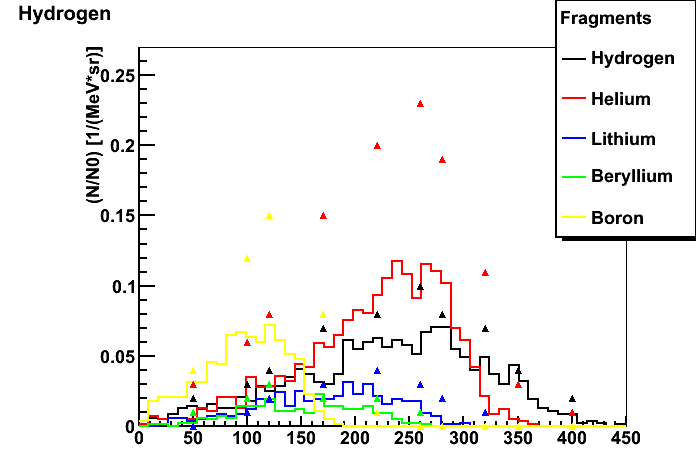
\includegraphics[width=0.9\textwidth]{images/fragmentEnergyDistr.png}  
\caption{\label{fig:fragmentEnergyDistr} Fragment energy distribution. Triangles from experimental data, solid bars simulated. Water phantom thickness was 27.9cm (slightly beyond the Bragg-peak)}
\end{center}
\end{figure}
\begin{figure}[!h] 
\begin{center}
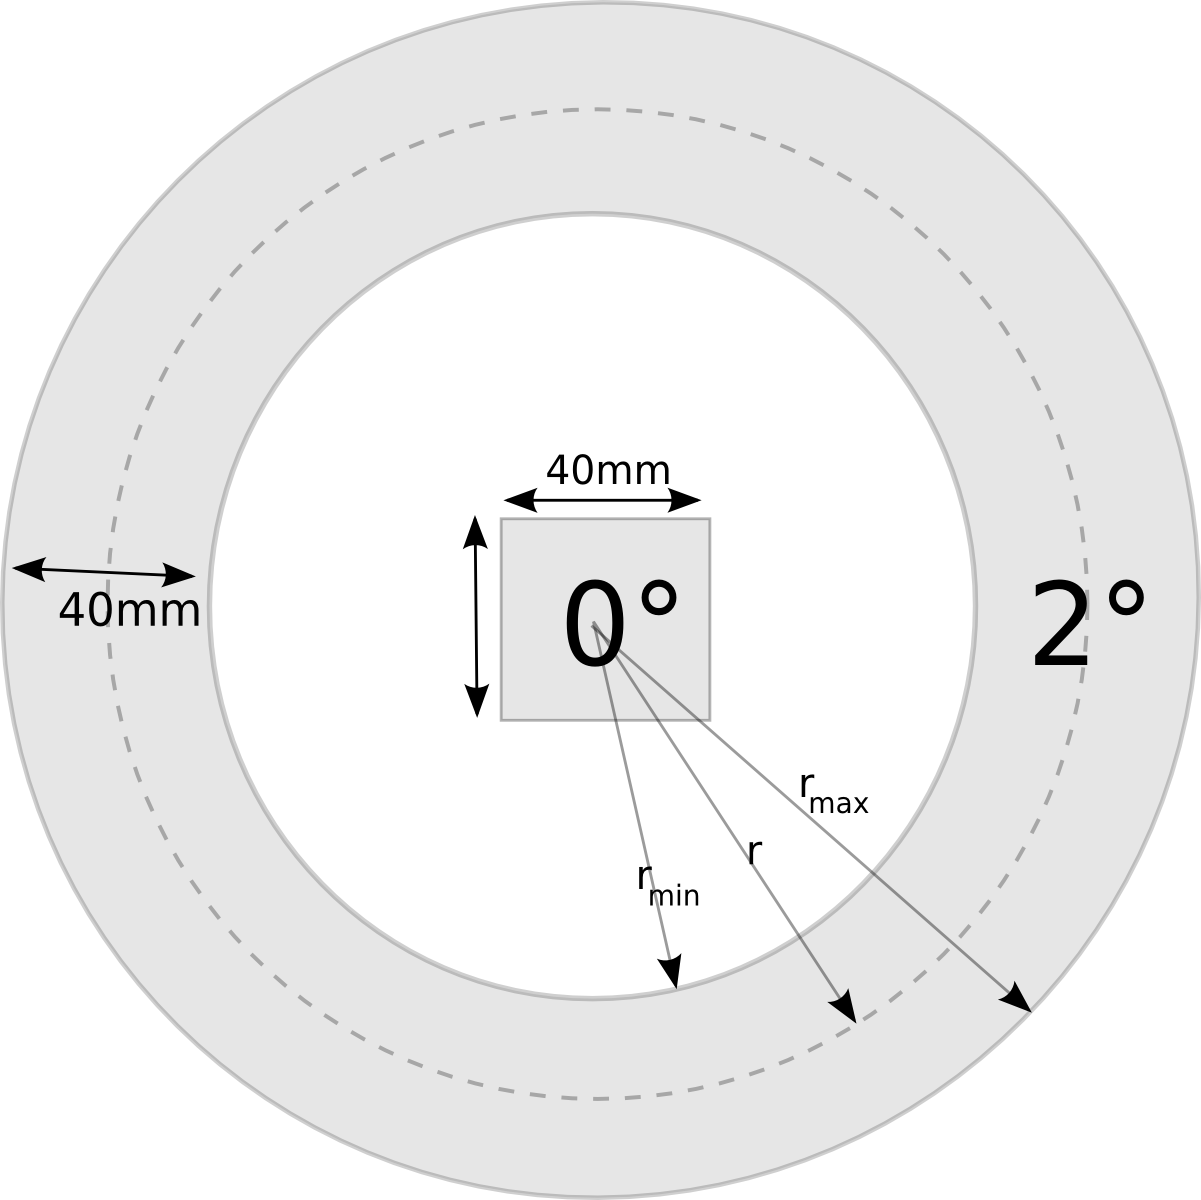
\includegraphics[width=0.6\textwidth]{images/annulus.png}  
\caption{\label{fig:annulusesExplained} Schematic picture of read-out area for charged fragments. Zero degrees is read out from a square detector while larger than zero degree angles are read out with consecutive largening circle annuluses where the middle radius $r$ is seen t tht scattering angle from the middle of the water phantom. The Annulus width is determined trigonometrically for each angle of analysis in order to correspond to the solid angle covered by H1.}
\end{center}
\end{figure}

A detector distance of 298.5cm was used as described by Haettner \cite[fig 5.1]{ehaettner} . In the experiment the H1 detector was moved and yields at different angles were recorded and plotted as a function of the angle at which the detector was seen. However, in order to increase effectivness of the simulation circle annuluses were used as detection areas at angles greater than zero. For the fragmentation at 0 degrees angle a square detection area was used. This approach is a slight approximation when it comes to small angles as the flux of the detection area may not be considered exactly similar to that of a square detector at that angle.

The annulus width a was determined so that it covered all of the solid angle that the detector rotated around the beam axis would cover. Thus the width of the annulus a is a function of $\phi$ acording to the relation. $a(\phi) = \text{H1 Sidelength} \times (\cos(\phi)+ \cot(\frac{\pi}{2} - \phi - \Delta\phi)\sin(\phi))$ where $\Delta\phi = \arctan(\frac{2 \times \text{Scattering distance}}{\cos(\phi) \times \text{H1 Sidelength}})$ is the angle subtended by $r$ to $r_{min}$ and $r_{max}$ respectively.

Results were divided by the amount of events and normalized to the solid angle of the detection area.

A square detector at 0 degree angle forms the base of the pyramid where the beam source is at the top and the principal beam axis runs along the apex. Thus, the formula $\Omega_{square} = 4 \arcsin{\frac{s^2}{(4d^2+s^2)}}$ for the solid angle of a pyramid describes the solid angle subtended by the detector H1 with side-length s at distance d from the beam-source.

The annulus of a circle subtends the solid angle $\Omega_{annulus} = 2 \pi (\cos(\theta_{min}) - \cos(\theta_{max}))$. in this formula $\theta_{min}$ and $\theta_{max}$ corresponds to the angle that $r_{min}$ respectively $r_{max}$ are seen at in the middle of the water-phantom. The magnitude of these two angles was trigonometrically determined as functions of the measurement angle $\phi$.

%\begin{comment}
%Koska lupasin koordinoida speksien määärittelyn.
%voisit Gillis tehdä raporttiisi seuraavaksi alaluvun :
%'Characterization of the primary beam and experimental setup for the
%IAEA benchmark'
%Ennen kun rupeat rakentamaan Geant4 simulaatiota  voisit siis kerätä
%Emman työstä
%kaikki vaadittavat tiedot (etäisyydet, materiaalit, dimensiot, beamin
%tiedot) tähän lukuun.
%Tämän tekstin tulisi olla itsenäinen osa opinnäytetyötä jotta sen voi
%kätevästi jakaa muiden Monte-Carlo koodien edustajlle.
%(Näppärä taulukko ja kuva kuten gradussa selventävät asiaa.) Tekstin
%pohjalta pitää pystyä luomaan
%yksikäsitteisesti oikeanlainen Monte-Carlo koe jonka tuloksia sitten
%verrataan Emman mittauksiin.

%doc/talk/images/inclSummary.png
%images/haettnersetup.png
%\end{comment}

\begin{itemize}
\item Experiment data from GSI
\item target description
\item Characterization and simulation of the beam (will be ignored, gaussian shape half-width fullheight HWFH assumed narrow pen beam - randomly pick in a small gaussian beam error perhaps - g4uniformrand-gaussian or check )
\item Simulation of detectors
\item Implementation details
\end{itemize}



\subsection{Analysis}
The simulation setup generates relatively little data. Thus an approach with separate analysis was chosen. All events hitting the detectors were recorded and suitable ones were chosen in ROOT. This section covers the analysis of the recorded events.

\subsection{Used parameters for runs.}
\begin{itemize}
 \item Fragment energydistribution: 500 000 events, cuts 0.4
 \item Angular distributions: one run per depth (5.9,15.9,27.9,31.2,31.4), 100 000 events.
 \item Beam shape, 10 000 events, reiterated until empirically the best fit was found
\end{itemize}


\section{Results and comparison to GSI data and other simulation models}

This work focused much on the fragments generated in the water phantom. Thus, much of the work has been put into analysing the different distributions of these fragments as they leave the water-phantom. In this section angular both angular and energy distributions will be presented for different water phantom thicknesses and they will be compared to data from E.Haettner. The thicknesses are chosen so that the distributions can be viewed for the beam both ahead and behind the Bragg peak.

\subsection{Beam shape\label{beamShapeAnalysis}}
The particle guns beam shape was set so that E.Haettner's measured 0 cm distance scattering of 4mm fwhm was duplicated. When this scattering experiment was repeated for the two other provided measurement points of 1m and 3m results were not in line with those of E.haettner. It was assumed further scattering not accounted for in the beam-source must have taken place. To compensate this a gaussian shaped stochastical error was introduced in the beam's momentum vector. This error was symmetrical in y and z and had the magnitude of $.1 \%$ of the x-component. This error was empirically chosen. The results are summarized in the table below.
 %permille sign, fix 
\begin{center}
 \begin{table}[h]
\begin{tabular}{cccc} %fixme:
\textbf{Distance} & \textbf{E.Haettner (hxv)} & \textbf{Straight incident beam} & \textbf{Added scattering} \\
0m &4x4 mm& 3.9 mm & 3.9 mm\\
1m &5x4 mm & 4.2 mm & 4.8 mm\\
3m &11x9mm& 5.2 mm & 9.0 mm\\
\end{tabular} 
\caption{\label{fig:beamFWHMtable} The beam FWHM as measured in experiment and reproduced in simulation and modified simulation.}
\end{table}
\end{center}

\subsection{Yields (0$^\circ$-10$^\circ$)}
E. Haettner has provided estimates for the yields inside 10 degrees angle. This estimate is based on fitting a normal distribution to low angles of the angular distribution and an exponential function to the larger angles. Thus numbers arep roduced for the total yield of each fragment in the 0$^\circ$-10$^\circ$ directions per incident carbon nucleon.

The same data was acquired through simulation. The below table summarizes the results.



\subsection{Energy distribution of fragments}
Events with energy greater than 45 MeV were picked as experimental data was unavailable at smaller energies. The data was normalized for bin-width (9MeV) and the solid angle of the square H1 detector with middlepoint at 0 degree angle from the mean direction of the beam.

The shape of the results are mostly in line with the experimental data. However, the yields of helium is clearly smaller than that of experimental results. This pheomena is repeated also in other water-depths. Further results are listed in the appendices.


\subsection{Angulara distribution of fragments}
\begin{figure}[!h] 
\begin{center}
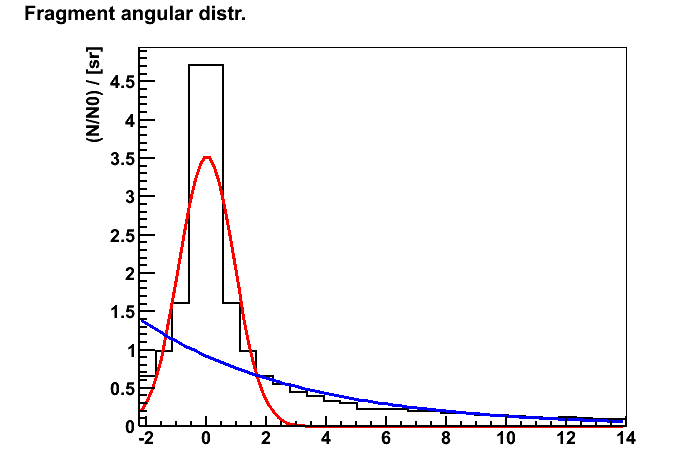
\includegraphics[width=0.5\textwidth]{images/plots/angularDistributions/equlBinnedHydrogen279.png}  
\caption{\label{fig:binnedHydrogen} Hydrogen scattering angles binned with equal bin lengths. Gaussian and exponential fit applied.}
 \end{center}
 \end{figure}
The angular distributions of the data were simulated for a number of phantom-depths before and after the Bragg peak at about 27cm. Results were normalized per number of incident ions and solid angle. The results we're plotted against E. Haettners data and are viewble in the appendices~\cite{AppendixA}. Results for $\phi \in [0,\arctan(\frac{\text{Detector sidelength}}{2 \times \text{Scattering distance}}) \approx 0.4]$ were discarded in the plots due to their ambiguous nature, due to the annulus-based read-out angle aproximation being misleading at angles where $r_{min} = 0$.

The obvious difference to the experimental data is the clearly lower yields at low angles. This relation is apparent for almost all depths and fragments that were analyzed. The difference seems to be accentuated for the lighter fragments.  As beam attenuation data matches well the lack of forward yield may indicate that the simulation models scattering of fragments is too isotropic.

In figure~\ref{fig:binnedHydrogen} the angular distributions were recorded so that all fragments were binned in an equal angle bin histogram. This exemplifies well how the distribution is at small angles best described by a Gaussian shape while at larger angles an exponential function is a better fit. The need for a two-component model has been observed by several authors (Haettner~\cite{ehaettner}, Gunzert-Marx~\cite{gunzert-marx}, Golovkov~\cite{golovkov}). However as this approach differs from the one used by E. Haettner this graph is not comparable to her results. The results in the appendices mimic that approach by having variable size bins.

All in all the results seem fair for a hadronic Monte-Carlo model.

\subsection{Angular energy distribution of fragments}

The angular energy plots were normalized for solid angle, number of events and bin-width. Although also here it is obvious the yields are too small at small angles, the shape of the distribution seems a satisfactory match. Similar indications were obtained with other fragments and depths as well. However, this graph verifies the missing forward-yield's energy is equally distributed to the rest of the detected fragments.

Data for the energy distributions can here only be compared to a copy directly from the publication due to data-files for this distribution not being available to the author at the time of writing.

\begin{figure}[!ht]
\centering
\subfigure[Experimental data]{
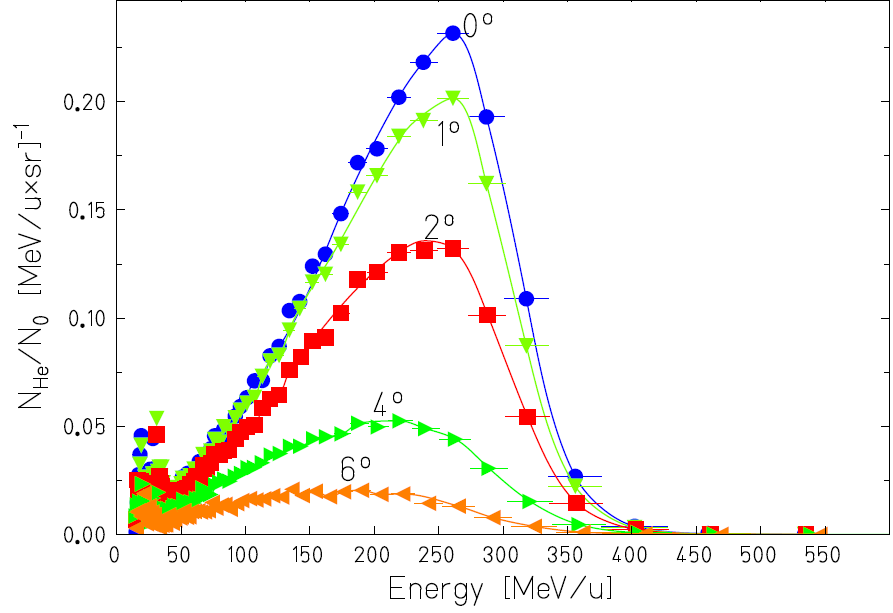
\includegraphics[width=0.45\textwidth]{images/plots/angularEnergyDistributions/EHaettnerDataForAEDistrib1.png}
\label{fig:EHaettnerDataForAEDistrib1}
}
\subfigure[Simulation data]{
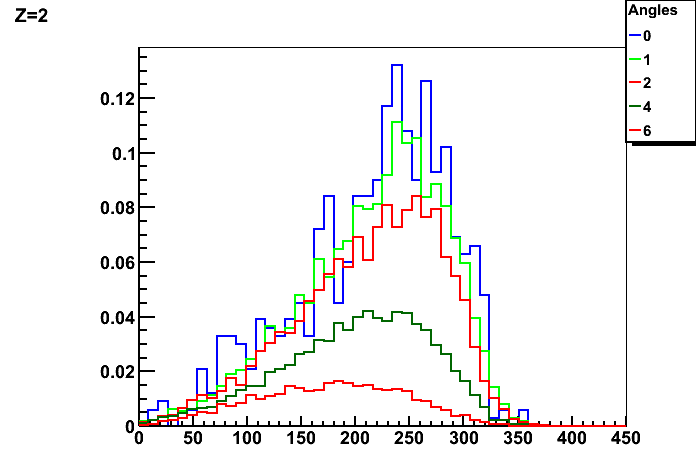
\includegraphics[width=0.45\textwidth]{images/plots/angularEnergyDistributions/AEDistrib2.png}
\label{fig:AEDistrib1}
}
\label{fig:subfigureExample}
\caption[Optional caption for list of figures]{The angular energy distributions with a 27.9cm water phantom. Although the yields at small angles seems to be clearly smaller in simulations than in experiments the distribution of energies is a fair match.}
\end{figure}

\subsection{Bragg curve}
The Bragg peak was measured from the simulation data to be located at $27.16 \pm 0.05 cm$ which is a rather good match with experimental result of 27.46cm. This difference alone was not deemed as sufficient to explain the missing forward-yield.

The greatest difference is the average ionization per meter in water, which is about 50 percent larger in the experimental data. %fixme, is this really so

It is also notable the results are very similar to those acquired with the FLUKA code by 

\begin{figure}[h] 
\begin{center}
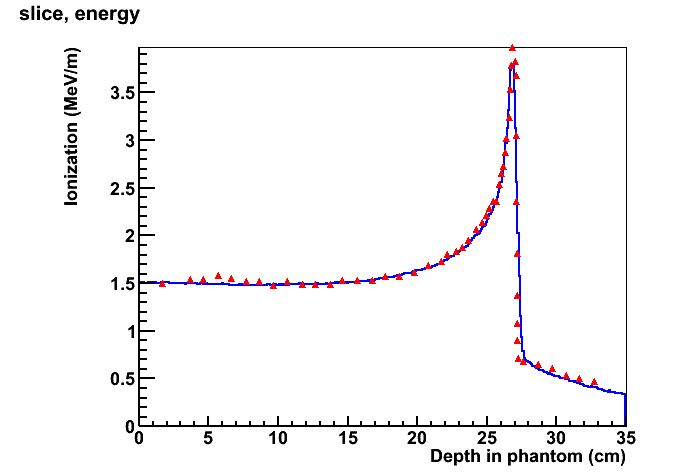
\includegraphics[width=0.9\textwidth]{images/plots/braggPeak/braggPeakComparisonToData.png}  
\caption{\label{fig:braggPeakCompared} Comparison with simulation bragg peak (blue) and experimental data (red)}
 \end{center}
 \end{figure}


\section{Conclusion and outlook}
Considering the relative quality of Monte Carlo models for hadronic physics it may be concluded that results all in all were pretty well in line with the experimental data. However, it is clear that there are certain discrepancies are viewable in the results which are not within the error-margins of the experimental work.

Further work is needed to determine the cause of these lacks in yields. As a good starting hypothesis one may choose to research the isotropicity of the evaporation model, because the missing yields at low angles is especially apparent for light fragments.

For this work the detectionvoxels in the phantom need to be changed to the \textit{G4SensitiveDetector} type from \textit{G4PrimitiveDetector}. This change will allow better analysis of what happens inside the water phantom instead of just the analysis of the resulting fragments that was focused on in this paper.

The experimental data pool of carbon beams is rather limited, and the paper by E.Haettner used as reference in this article is one of the more thorough ones with relatively good possibilities for recreating the experiment and compare the data. However, there remains a number of things in this experiment that were not recreatable in the simulation code.

The author hopes by this paper to provide a contribution to the pool of carbon treatment related simulation analysises, and ease the development of models.

The author also studied others models for hadronic simulations. The original intent of this paper was t operform the simulations with INCL and ABLA code. However, the newest release of the INCL code was not released at the time of writing and thus support for light nucleus interactions was not included. This work is therefore left for the future, with a good adaptable GEANT4b framework and related ROOT analysis scripts. The theoretical basis of INCL and ABLA is also described in appendix \refname{appendixincltheory}


\bibliographystyle{plain} \bibliography{refs.bib} 

%%%%% Liitteet 
\appendix 

\clearpage
\addcontentsline{toc}{section}{Appendix A: Angular Distributions of charged fragments.}
\section*{Appendix A \label{AppendixA}: Angular Distributions of charged fragments.\label{AngularDistributionAppendix}}

%% Liitteiden kaavat, taulukot ja kuvat numeroidaan omana kokonaisuutenaan
\renewcommand{\theequation}{A\arabic{equation}}
\setcounter{equation}{0}  
\renewcommand{\thefigure}{A\arabic{figure}}
\setcounter{figure}{0}
\renewcommand{\thetable}{A\arabic{table}}
\setcounter{table}{0}
\renewcommand\thesection{A}
\setcounter{section}{1}

\subsection{Hydrogen}
\begin{figure}[!h]
\centering
\subfigure[5.9cm, very much differing yields. However Haettner gives large uncertainty for values due to carbon ion interference in data.]{
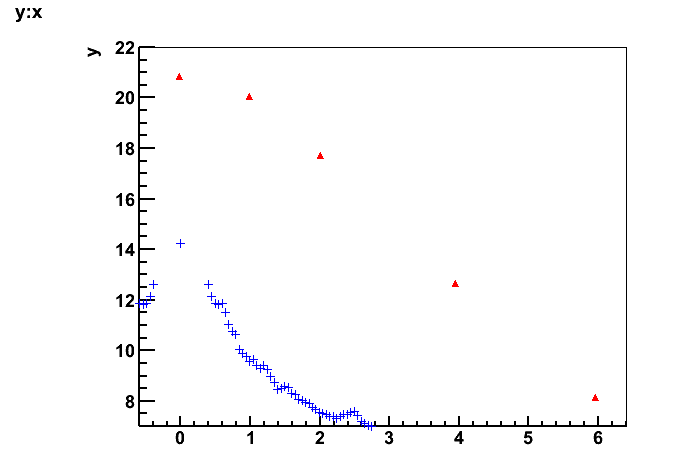
\includegraphics[width=0.45\textwidth]{images/plots/angularDistributions/AD_59_1_N.png}
\label{fig:AD_5.9_1_N}
}
\subfigure[15.9cm]{
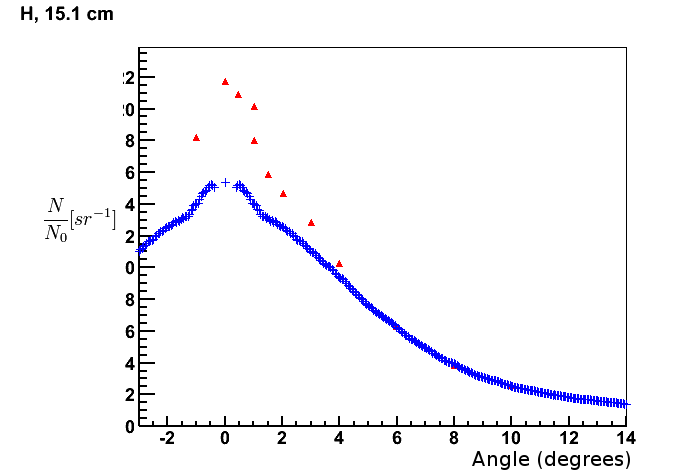
\includegraphics[width=0.45\textwidth]{images/plots/angularDistributions/AD_159_1_N.png}
\label{fig:AD_15.9_1_N}
}
\subfigure[27.9cm]{
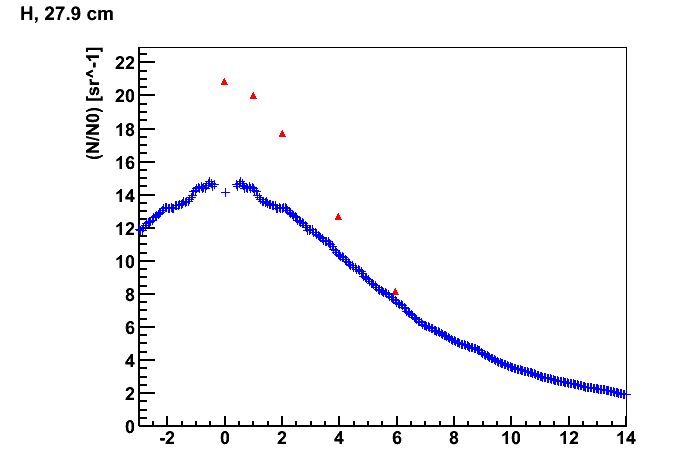
\includegraphics[width=0.45\textwidth]{images/plots/angularDistributions/AD_279_1_N.png}
\label{fig:AD_27.9_1_N}
}
\subfigure[31.2cm]{
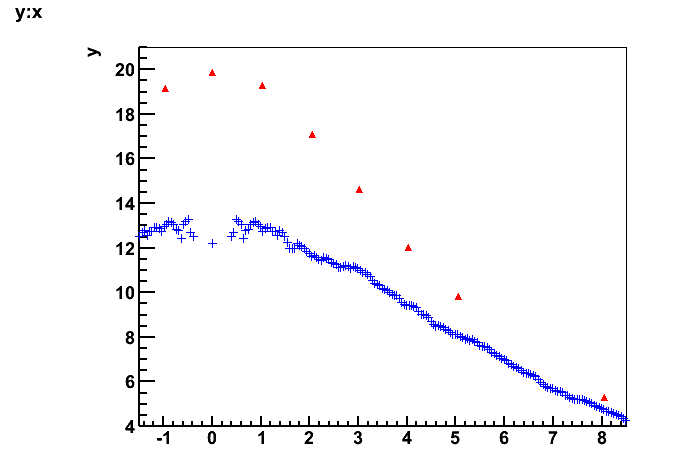
\includegraphics[width=0.45\textwidth]{images/plots/angularDistributions/AD_312_1_N.png}
\label{fig:D_31.2_1_N}
}
\subfigure[34.7cm]{
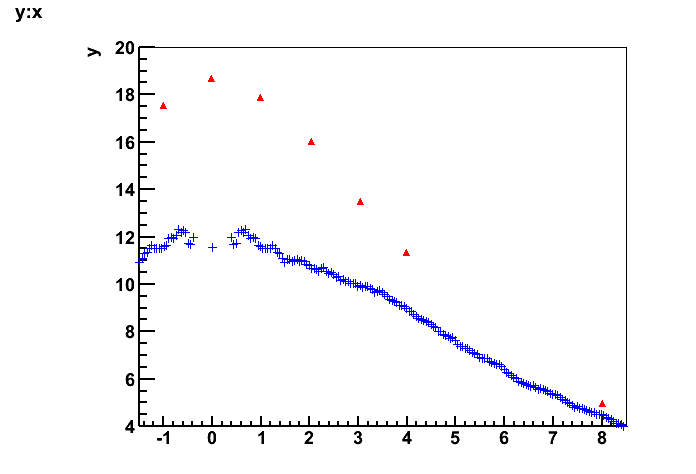
\includegraphics[width=0.45\textwidth]{images/plots/angularDistributions/AD_347_1_N.png}
\label{fig:D_34.7_1_N}
}
\label{fig:subfigureExample}
\caption[Optional caption for list of figures]{he angular distribution plots as described in \cite{AngularDistributionText}. The red triangles represent data from E. Haettner \cite{ehaettner}, and the blue crosses are calculated through the described monte carlo simulation.}
\end{figure}
\clearpage
\subsection{Helium}
\begin{figure}[!ht]
\centering
\subfigure[5.9cm]{
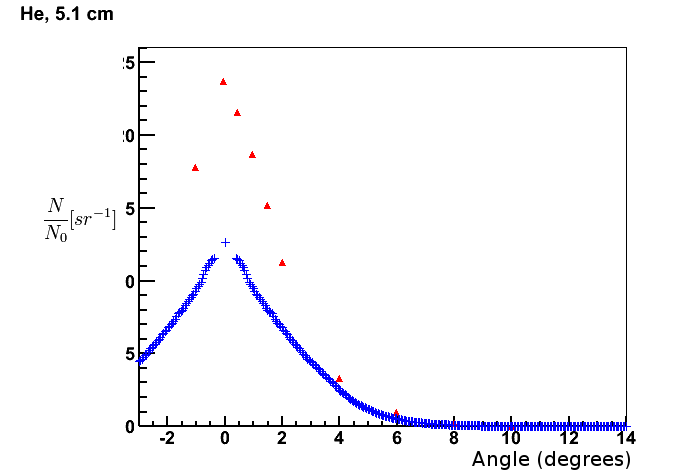
\includegraphics[width=0.45\textwidth]{images/plots/angularDistributions/AD_59_2_N.png}
\label{fig:AD_5.9_2_N}
}
\subfigure[15.9cm]{
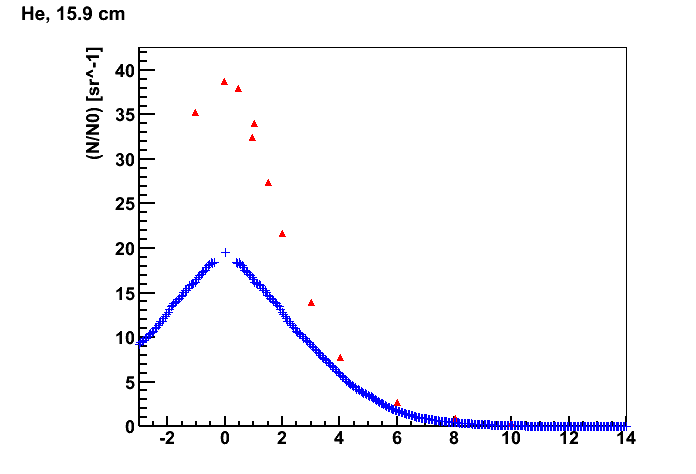
\includegraphics[width=0.45\textwidth]{images/plots/angularDistributions/AD_159_2_N.png}
\label{fig:AD_15.9_2_N}
}
\subfigure[27.9cm]{
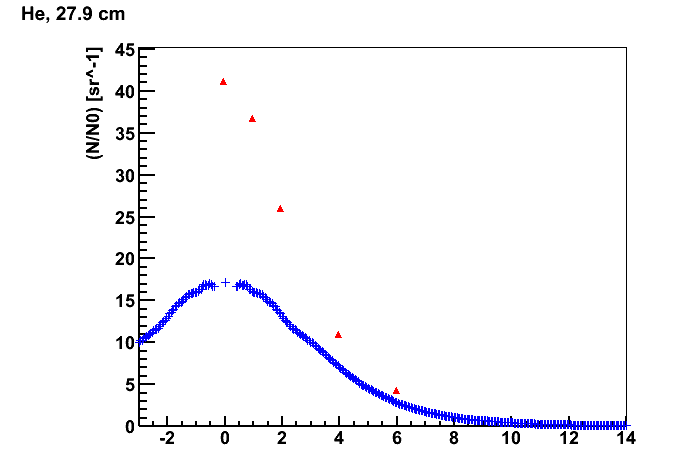
\includegraphics[width=0.45\textwidth]{images/plots/angularDistributions/AD_279_2_N.png}
\label{fig:AD_27.9_2_N}
}
\subfigure[31.2cm]{
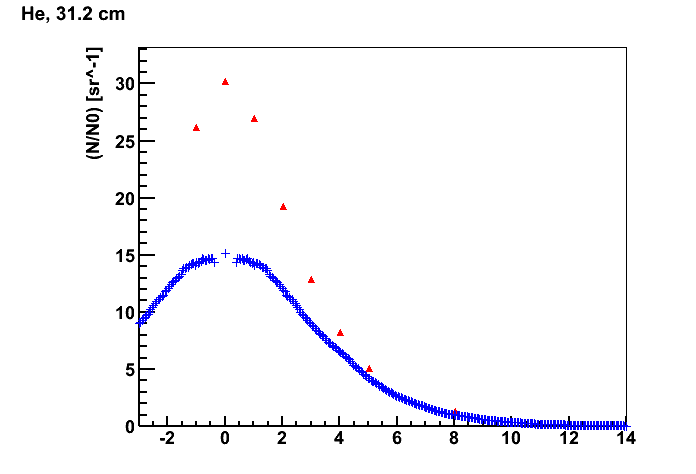
\includegraphics[width=0.45\textwidth]{images/plots/angularDistributions/AD_312_2_N.png}
\label{fig:D_31.2_2_N}
}
\subfigure[34.7cm]{
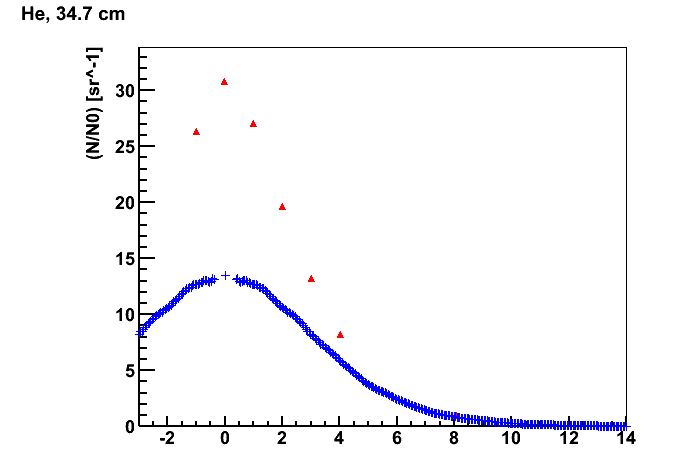
\includegraphics[width=0.45\textwidth]{images/plots/angularDistributions/AD_347_2_N.png}
\label{fig:D_34.7_2_N}
}
\label{fig:subfigureExample}
\caption[Optional caption for list of figures]{the worst correlation is for \subref{fig:AD_5.9_1_N}}
\end{figure}
\clearpage
\subsection{Lithium}
\begin{figure}[!ht]
\centering
\subfigure[5.9cm]{
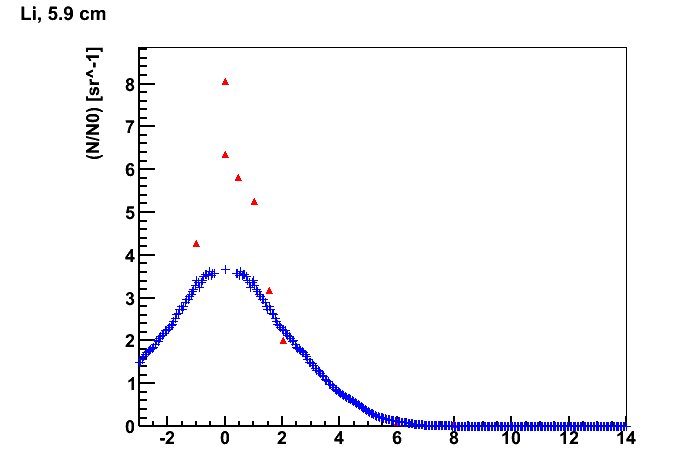
\includegraphics[width=0.45\textwidth]{images/plots/angularDistributions/AD_59_3_N.png}
\label{fig:AD_5.9_3_N}
}
\subfigure[15.9cm]{
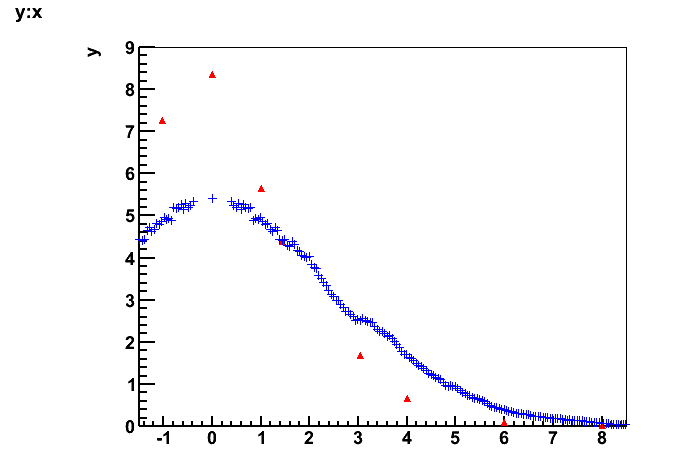
\includegraphics[width=0.45\textwidth]{images/plots/angularDistributions/AD_159_3_N.png}
\label{fig:AD_15.9_3_N}
}
\subfigure[27.9cm]{
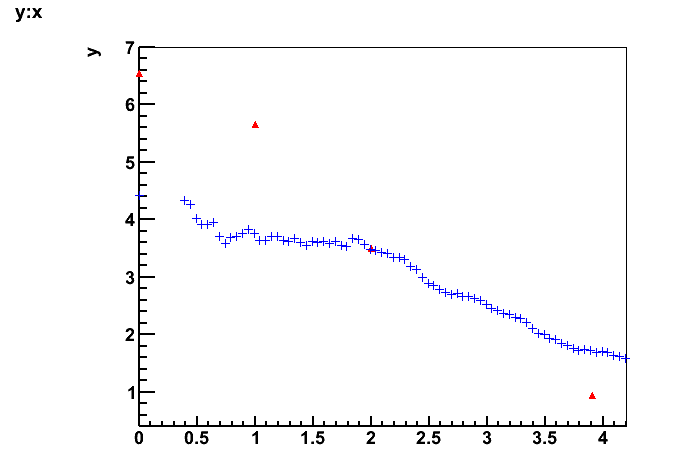
\includegraphics[width=0.45\textwidth]{images/plots/angularDistributions/AD_279_3_N.png}
\label{fig:AD_27.9_3_N}
}
\subfigure[31.2cm]{
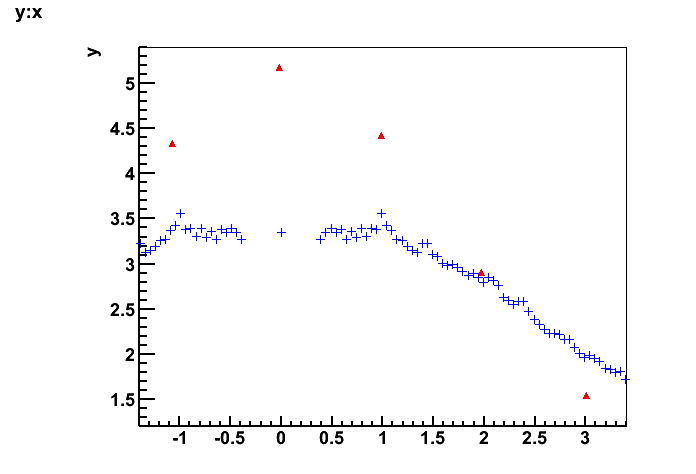
\includegraphics[width=0.45\textwidth]{images/plots/angularDistributions/AD_312_3_N.png}
\label{fig:D_31.2_3_N}
}
\subfigure[34.7cm]{
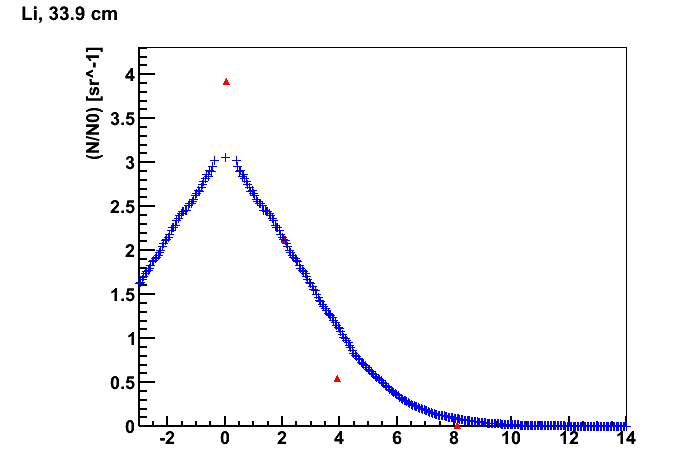
\includegraphics[width=0.45\textwidth]{images/plots/angularDistributions/AD_347_3_N.png}
\label{fig:D_34.7_3_N}
}
\label{fig:subfigureExample}
\caption[Optional caption for list of figures]{}
\end{figure}
\clearpage
\subsection{Beryllium}
\begin{figure}[!ht]
\centering
\subfigure[5.9cm]{
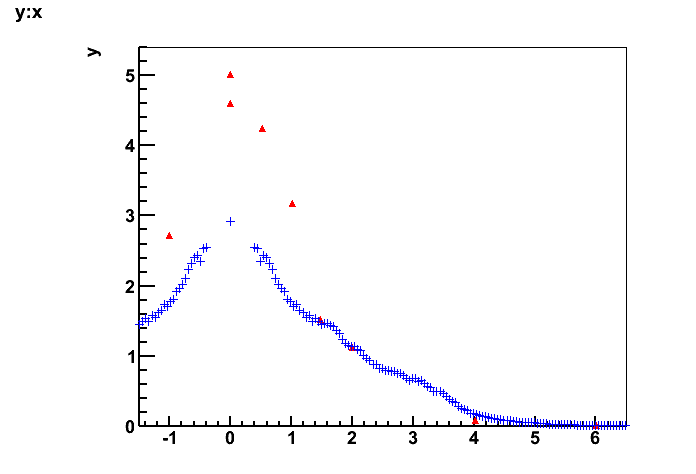
\includegraphics[width=0.45\textwidth]{images/plots/angularDistributions/AD_59_4_N.png}
\label{fig:AD_5.9_4_N}
}
\subfigure[15.9cm]{
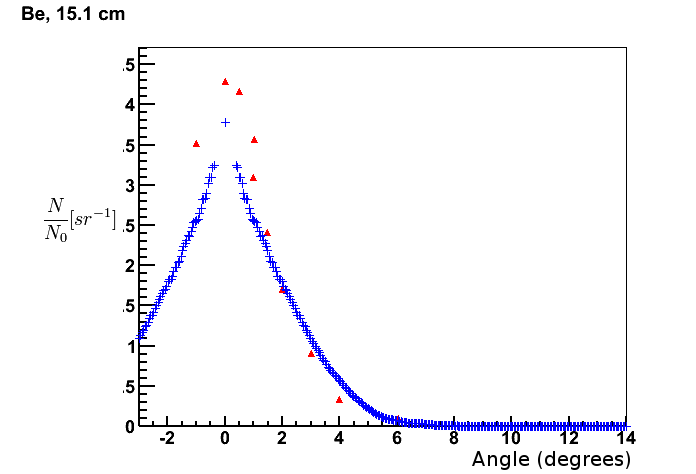
\includegraphics[width=0.45\textwidth]{images/plots/angularDistributions/AD_159_4_N.png}
\label{fig:AD_15.9_4_N}
}
\subfigure[27.9cm]{
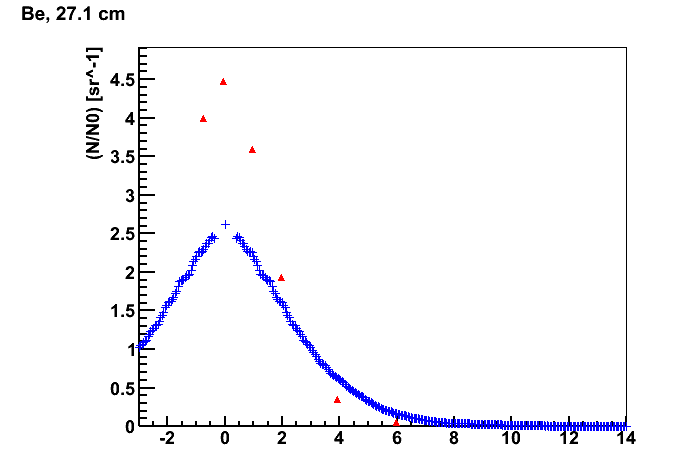
\includegraphics[width=0.45\textwidth]{images/plots/angularDistributions/AD_279_4_N.png}
\label{fig:AD_27.9_4_N}
}
\subfigure[31.2cm]{
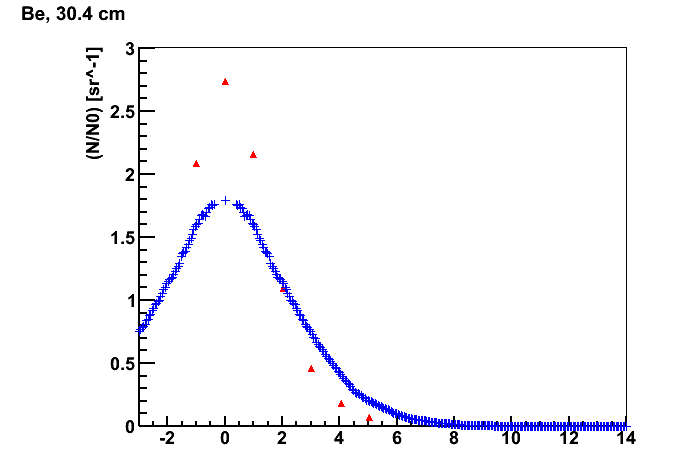
\includegraphics[width=0.45\textwidth]{images/plots/angularDistributions/AD_312_4_N.png}
\label{fig:D_41.2_4_N}
}
\subfigure[34.7cm]{
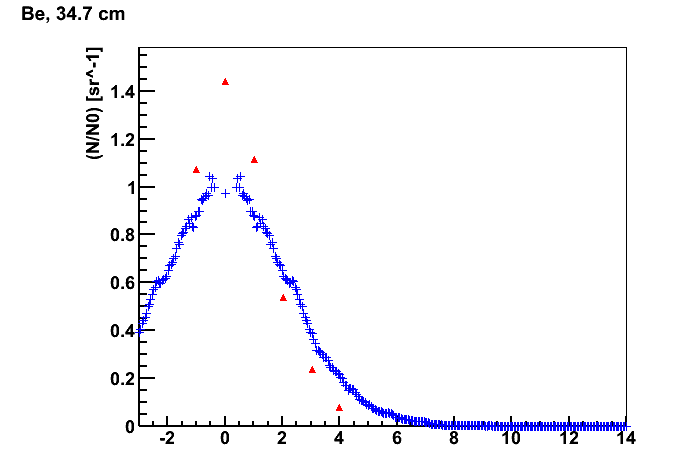
\includegraphics[width=0.45\textwidth]{images/plots/angularDistributions/AD_347_4_N.png}
\label{fig:D_43.7_4_N}
}
\label{fig:subfigureExample}
\caption[Optional caption for list of figures]{}
\end{figure}
\clearpage
\subsection{Boron}
\begin{figure}[!ht]
\centering
\subfigure[5.9cm]{
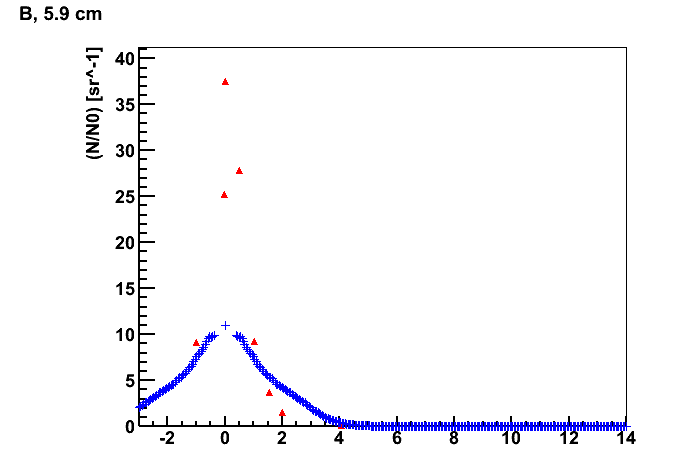
\includegraphics[width=0.45\textwidth]{images/plots/angularDistributions/AD_59_5_N.png}
\label{fig:AD_5.9_5_N}
}
\subfigure[15.9cm]{
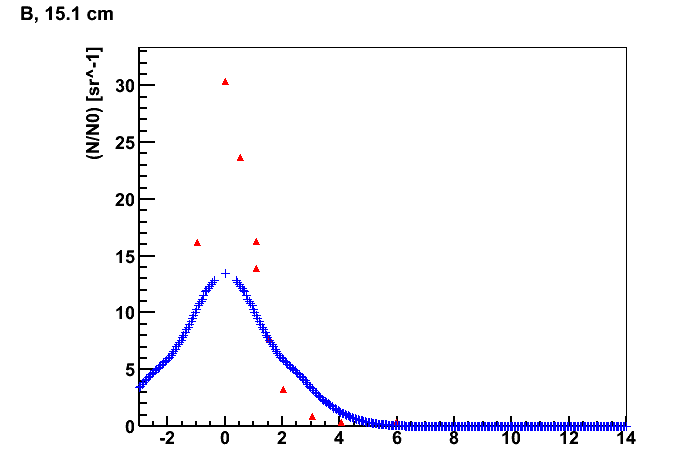
\includegraphics[width=0.45\textwidth]{images/plots/angularDistributions/AD_159_5_N.png}
\label{fig:AD_15.9_5_N}
}
\subfigure[27.9cm]{
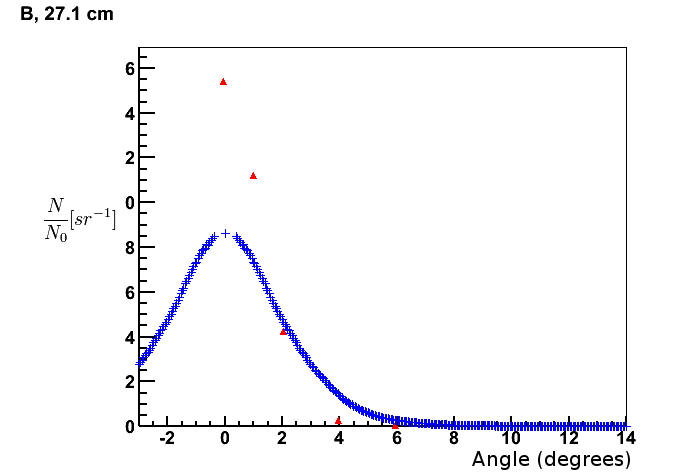
\includegraphics[width=0.45\textwidth]{images/plots/angularDistributions/AD_279_5_N.png}
\label{fig:AD_27.9_5_N}
}
\subfigure[31.2cm]{
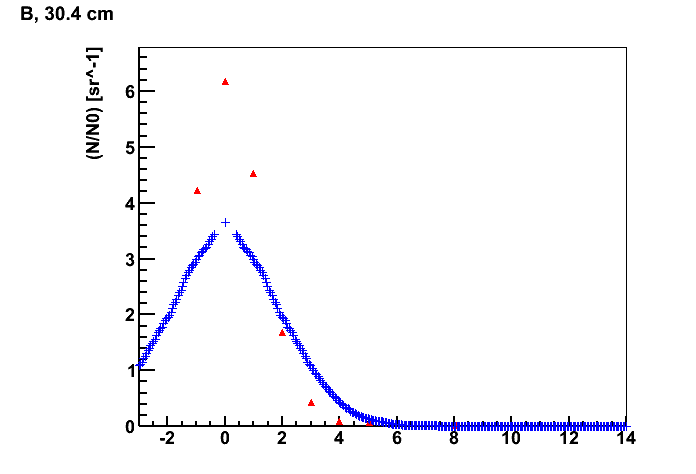
\includegraphics[width=0.45\textwidth]{images/plots/angularDistributions/AD_312_5_N.png}
\label{fig:D_31.2_5_N}
}
\subfigure[34.7cm]{
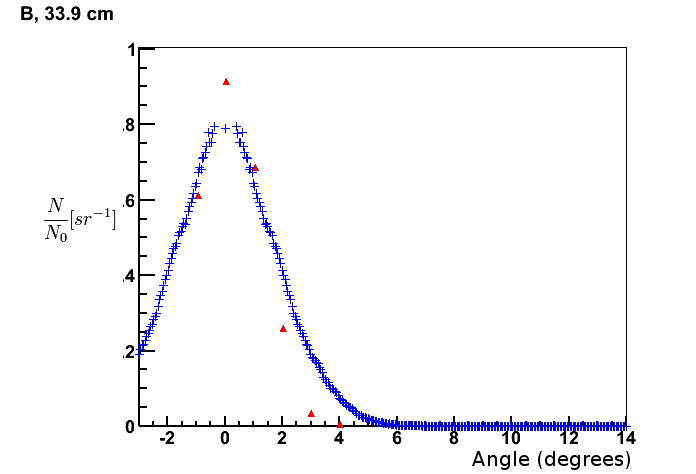
\includegraphics[width=0.45\textwidth]{images/plots/angularDistributions/AD_347_5_N.png}
\label{fig:D_34.7_5_N}
}
\label{fig:BoronAD}
\caption[Optional caption for list of figures]{}
\end{figure}
\clearpage
\begin{itemize}
\item angular distribution plots
\item code examples
\item runtime log
\end{itemize}
\clearpage

\addcontentsline{toc}{section}{Appendix B: Theory of proposed alternative simulation models}
\section*{Appendix B \label{AppendixB}: Theory of proposed alternative simulation models}

%% Liitteiden kaavat, taulukot ja kuvat numeroidaan omana kokonaisuutenaan
\renewcommand{\theequation}{B\arabic{equation}}
\setcounter{equation}{0}  
\renewcommand{\thefigure}{B\arabic{figure}}
\setcounter{figure}{0}
\renewcommand{\thetable}{B\arabic{table}}
\setcounter{table}{0}
\renewcommand{\thesection}{B}
\setcounter{section}{1}
\section*{Theory of proposed alternative simulation models \label{appendixincltheory}}
\subsection{INCL}

INCL is a implementation of the Liège INC model. It is designed for use in the 200MeV-2GeV region where standard cross-section libraries no longer are sufficient. Containing only few free parameters INCL has proven predictive power.

INCL is called into action when Geant4 selects from available model an inelastic collision will take place. INCL then takes as parameters the beam-particle and the target nucleus. It then proceeds to randomly pick what type of collision will happen by selecting the impact parameter between zero and the the target nucleus radius. The impact parameter is defined as the perpendicular distance between the velocity of the projectile and the center of the nucleus it is approaching.

In the Liège INC model particles move in straight deterministic trajectories, which makes upcoming collisions practical to predict in the INCL code.
 The nucleus in INCL is modelled as fermi-gas in a Woods-Saxon potential. %fixme woods-saxon
 The Woods-Saxon potential barrier gives a potential barrier that is smooth. Thus, in the INCL code the nucleons are randomly picked from a Woods-Saxon probability density distribution.

\begin{equation}
\rho(r) = \begin{cases}
\frac{\rho_{0}}{1+\exp({\frac{r-R_{0}}{a}})} & 0 < r < R_{max} \\
0 & \text{otherwise}
\end{cases}
\label{WoodsSaxon2}
\end{equation}

If the energy of the bullet particle breaks the nucleus potential barrier and enters the nucleus several binary collisions between participating nucleons will take place, smaller particles may be emerge out from the nucleus. Spectator particles may move around the nucleus and bounce off its edges by reflection, however, they will not leave the nucleus.

The kinetics of the model are bound by the physical laws of conservation of baryon number, charge, energy, momentum and angular momentum and respect the Pauli blocking principle. Furthermore, pion-production is governed through the relation of $NN \rightleftharpoons N \Delta, \Delta \rightleftharpoons N\pi$ (with a stochastically determined mass for $\Delta$).

The major free parameter of the INCL code is the stopping-time; the time before thermal equilibrium can be assumed and thus the process handed over to the evaporation and fission phase. The INCL code has chosen the stopping time as a suitable function of the target nucleus size so that $$t_{stop} = f_{stop}t_{0}(\frac{A_T}{208})^{0.16},$$ where $f_{stop} = 1.0$. The stopping-time of INCL4 is considerably longer than for many models where discrete potential barriers are defined for the nucleus.

A further discussion of the theoretical basis of the Liège INC model and INCL code is available in references ~\cite{PhysRevC.66.044615,iia}.

\begin{figure}[ht]
\begin{center}
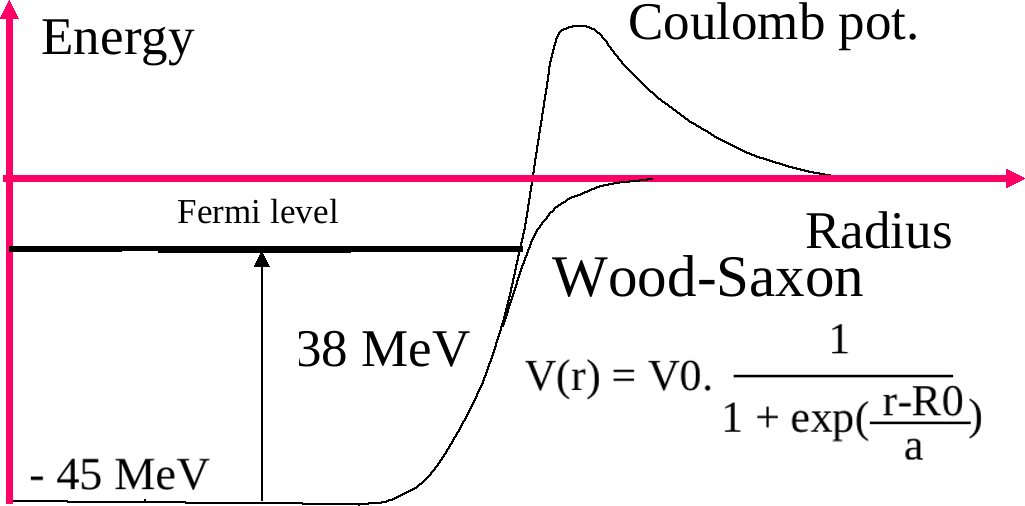
\includegraphics[width=0.3\textwidth]{images/inclPotential.png}  
\caption{\label{fig:inclpotential} Schematic of the potential model used by the INCL-model.}
 
 \end{center}
 \end{figure}


\subsection{ABLA}

The ABLA code has been developed at the GSI facility in Darmstadt, Germany. Its principal developers being K-H.~Schmidt and A.~Kelic. It is a Monte-Carlo code based on a data-set {\tt G4ABLADATA} distributed alongside the code. ABLA takes as input nucleus parameters, excitation energy, mass number, charge number and nucleus spin. It then calculates on the basis of this data the probabilities for different fission or evaporation events taking place according to statistical distributions obtained from experiments and phenomenology.

ABLA comes with two different fission models SimFis3 and SimFis18. These models are based on the proven PROFI-model also developed at GSI darmstadt. ABLA selects between competitive fission and evaporation processes as described in the flowchart~\ref{fig:ablatable}.

\begin{figure}[h] 
\begin{center}
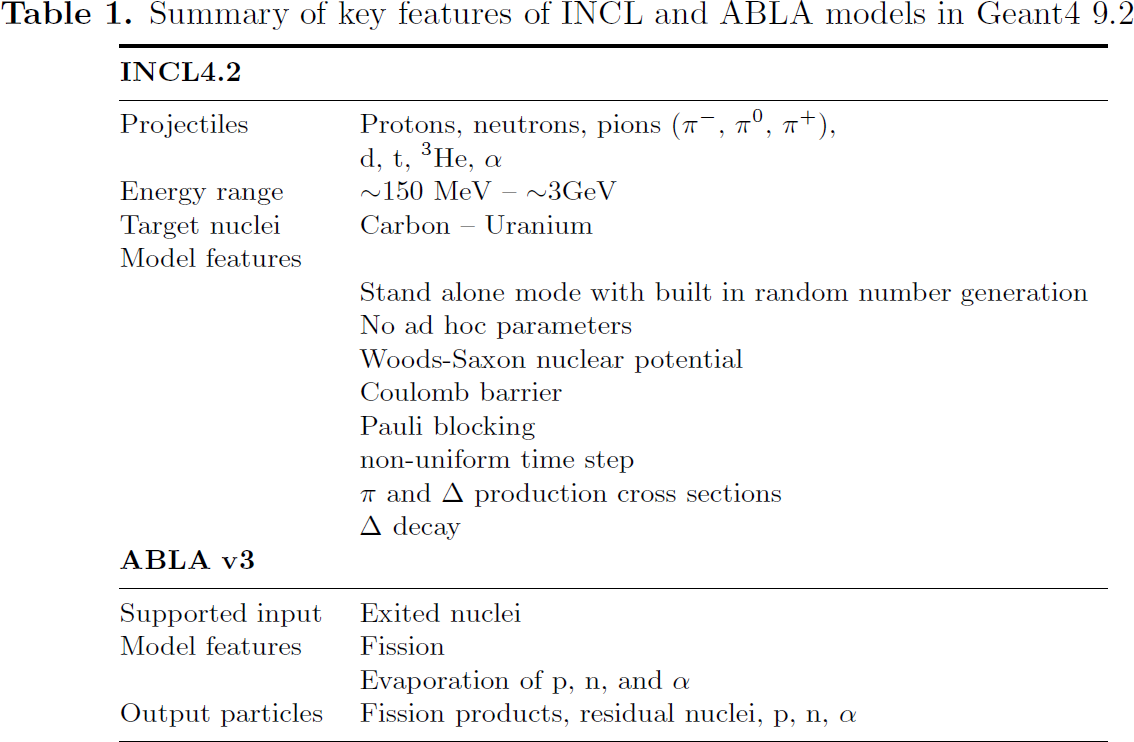
\includegraphics[width=1\textwidth]{images/inclSummary.png}  
\caption{\label{fig:inclpotential}}
 
 \end{center}
 \end{figure}

%fixme, add another picture with data

\begin{figure}[h] 
\begin{center}
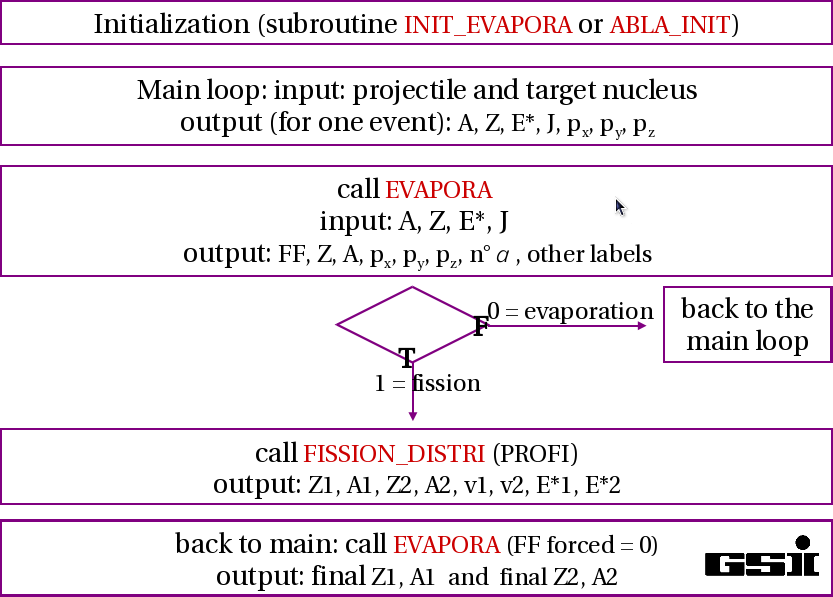
\includegraphics[width=0.6\textwidth]{images/AblaTable.png}[h]  
\caption{\label{fig:ablatable} General flow of ABLA submodels.}
 
 \end{center}
 \end{figure}
\begin{figure}[h] 
\begin{center}
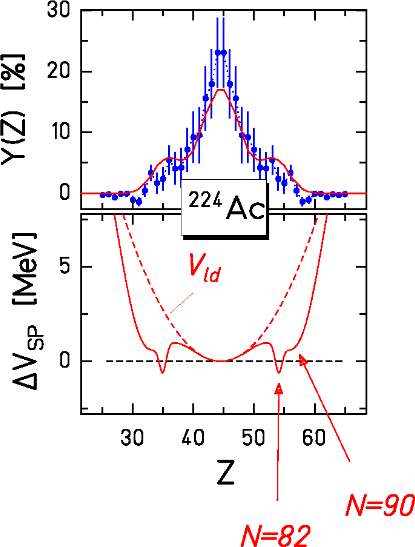
\includegraphics[width=0.3\textwidth]{images/AblaHumps.png}[h]  
\caption{\label{fig:ablahumps} ABLA symmetric (solid line) and antisymmetric (dashed line) fission plots.}
 
 \end{center}
 \end{figure}

A further discussion of the theoretical basis of the ABLA code is available in references ~\cite{ablatalk,iia}.
%fixme add another ABLAsource

\clearpage

\addcontentsline{toc}{section}{Appendix C: Log of work}
\section*{Appendix C \label{AppendixC}: Log of work}

%% Liitteiden kaavat, taulukot ja kuvat numeroidaan omana kokonaisuutenaan
\renewcommand{\theequation}{C\arabic{equation}}
\setcounter{equation}{0}  
\renewcommand{\thefigure}{C\arabic{figure}}
\setcounter{figure}{0}
\renewcommand{\thetable}{C\arabic{table}}
\setcounter{table}{0}
\renewcommand{\thesection}{C}
\setcounter{section}{1}
\section*{Log of work \label{logofwork}}

\subsection{Improving usability through messenger macro commands}
The first action task taken in this work was to implement means to speed up the use of the analysis model by means of messenger macro commands that would let the user change geometry setup inbetween runs without needing to compile the entire simulation again.

Macro commands are itnerpreted by the code, and are sent to the simulation and Geant4 through a specific messenger class. The features implemented through macro commands were
\begin{itemize}
 \item Ability to run multiple runs in one macro file, so that output is saved in separate root-files.
\item Ability to change the thickness of the water phantom, in such a way that all other parts of the geometry are changed as well to acustom the new phantom.
\item Ability to control the scoring area in the phantom and what is scored through command-based scoring.
\end{itemize}


So as aen example the user can give a command according to the following syntax.
\scriptsize
\begin{verbatim}
/analysis/setFileName <user-defined name>.root
\end{verbatim}
\normalsize

The implementation was done by creating an analysismessenger inheriting functionality from \textit{G4UImessenger}. An object of the type \textit{HadrontehrapyAnalysisMessenger} was created in the \textit{AnalysisManager}.


\scriptsize
\begin{verbatim}
class HadrontherapyAnalysisFileMessenger: public G4UImessenger
{
  public:
    HadrontherapyAnalysisFileMessenger(HadrontherapyAnalysisManager*);
   ~HadrontherapyAnalysisFileMessenger();
    
    void SetNewValue(G4UIcommand*, G4String);
    
  private:
    HadrontherapyAnalysisManager* AnalysisManager;
\end{verbatim}
\normalsize
\begin{figure}[h] 
\begin{center}
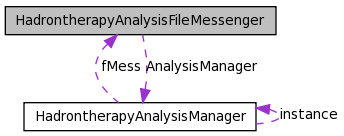
\includegraphics[width=0.3\textwidth]{images/setFileNameMessenger_1.png}  
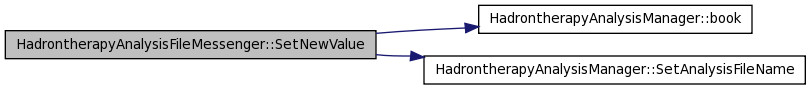
\includegraphics[width=0.7\textwidth]{images/setFileNameMessenger_2.png}  
\caption{\label{fig:messengerUML} UML diagrams for messen ger class}
 
 \end{center}
 \end{figure}

\end{document}



